%% ----------------------------------------------------------------
%% Thesis.tex -- MAIN FILE (the one that you compile with LaTeX)
%% ---------------------------------------------------------------- 

% Set up the document
\pdfminorversion=7
\documentclass[a4paper, 11pt, oneside]{Thesis}  % Use the "Thesis" style, based on the ECS Thesis style by Steve Gunn
\graphicspath{Figures/}  % Location of the graphics files (set up for graphics to be in PDF format)

% Include any extra LaTeX packages required
\usepackage[square, numbers, comma, sort&compress]{natbib}  % Use the "Natbib" style for the references in the Bibliography
\usepackage{verbatim}  % Needed for the "comment" environment to make LaTeX comments
\usepackage{vector}  % Allows "\bvec{}" and "\buvec{}" for "blackboard" style bold vectors in maths
\usepackage{acronym}
\usepackage[final]{pdfpages}
%\usepackage[hidelinks]{hyperref}
%\hypersetup{colorlinks=false}  % Colours hyperlinks in blue, but this can be distracting if there are many links
\hypersetup{
colorlinks = true,
hidelinks = true
}
%\hypersetup{
%    colorlinks,
%   % linkcolor={red!50!black},
%    linkcolor={black},
%    citecolor={blue!50!black},
%    urlcolor={blue!80!black}
%}
%% ----------------------------------------------------------------
\begin{document}
\frontmatter      % Begin Roman style (i, ii, iii, iv...) page numbering

% Set up the Title Page
\title{Machine Learning Based Restaurant Location Analysis in Hamburg}
\authors  {
			\texorpdfstring
            {\href{https://www.linkedin.com/in/vincent-meyer-zu-wickern-705b9610a/}{Vincent Meyer zu Wickern}}
            {Vincent Meyer zu Wickern},
            		\texorpdfstring
            {\href{https://www.linkedin.com/in/sachin-kumar-887aa953/}{Sachin Kumar}}
            {Sachin Kumar}, 
			\texorpdfstring
            {\href{}{Viet-Hung Vu}}
            {Viet-Hung Vu}
 	}

            
            
\addresses  {\groupname\\\deptname\\\univname}  % Do not change this here, instead these must be set in the "Thesis.cls" file, please look through it instead
\date       {\today}
\subject    {}
\keywords   {}

\maketitle
%% ----------------------------------------------------------------

\setstretch{1.5}  % It is better to have smaller font and larger line spacing than the other way round

% Define the page headers using the FancyHdr package and set up for one-sided printing
\fancyhead{}  % Clears all page headers and footers
\rhead{\thepage}  % Sets the right side header to show the page number
\lhead{}  % Clears the left side page header

\pagestyle{fancy}  % Finally, use the "fancy" page style to implement the FancyHdr headers


% Contribution to the project

\addtocontents{toc}{\vspace{1em}}  % Add a gap in the Contents, for aesthetics
\textbf{Contribution of authors to the project}

This paper was implemented in collaboration of all three authors. This implementation is available on Github under the link https://github.com/Vincentxyz/Hamburg\_Food\_Geo. The documentation of the paper was split among the three authors with the following chapters written by the respective authors:

\textbf{Vincent Meyer zu Wickern:}
\begin{itemize}
\item Abstract
\item chapter \ref{Introduction}: Introduction
\item section \ref{sec:Regression performance measures}: Regression of performance measures
\item chapter \ref{data_analysis}: Data analysis
\item section \ref{discussion_of_results}: Discussion of results
\item chapter \ref{Conclusion}: Conclusion
\end{itemize}

\textbf{Sachin Kumar}
\begin{itemize}
\item chapter \ref{factors_of_restaurant_success}: Factors of restaurant success
\item section \ref{sec:random_forest_regression}: Random forest regression
\item section \ref{Exploratory_data_analysis}: Exploratory data analysis
\end{itemize}

\textbf{Viet-Hung Vu}
\begin{itemize}
\item chapter \ref{Data sources}: Data sources
\item chapter \ref{Data extraction}: Data extraction
\end{itemize}


\clearpage

%% ----------------------------------------------------------------
% Declaration Page required for the Thesis, your institution may give you a different text to place here
%\Declaration{

\addtocontents{toc}{\vspace{1em}}  % Add a gap in the Contents, for aesthetics

\includepdf[pages=-,offset=30mm 0mm]{2019-02-17_Hamburg_Restaurant_Analysis_Declaration_of_Authorship.pdf}
%We,
%\begin{itemize}
%\item Vincent Meyer zu Wickern
%\item Sachin Kumar
%\item Viet-Hung Vu
%\end{itemize}
%, declare that this paper and the work presented in it are our own. We confirm that:
%
%\begin{itemize} 
%\item[\tiny{$\blacksquare$}] This work was done wholly or mainly while in candidature for a research degree at this University.
% 
%\item[\tiny{$\blacksquare$}] Where any part of this paper has previously been submitted for a degree or any other qualification at this University or any other institution, this has been clearly stated.
% 
%\item[\tiny{$\blacksquare$}] Where we have consulted the published work of others, this is always clearly attributed.
% 
%\item[\tiny{$\blacksquare$}] Where we have quoted from the work of others, the source is always given. With the exception of such quotations, this paper is entirely our own work.
% 
%\item[\tiny{$\blacksquare$}] We have acknowledged all main sources of help.
% 
%\item[\tiny{$\blacksquare$}] Where the paper is based on work done by ourselves jointly with others, we have made clear exactly what was done by others and what we have contributed ourselves.
%\\
%\end{itemize}
% 
% 
%Signed:\\
%\rule[1em]{25em}{0.5pt}  % This prints a line for the signature
%
%Signed:\\
%\rule[1em]{25em}{0.5pt}  % This prints a line for the signature
%
%Signed:\\
%\rule[1em]{25em}{0.5pt}  % This prints a line for the signature
% 
%Date:\\
%\rule[1em]{25em}{0.5pt}  % This prints a line to write the date
%\clearpage  % Declaration ended, now start a new page






%% ----------------------------------------------------------------
% The "Funny Quote Page"
%\pagestyle{empty}  % No headers or footers for the following pages
%
%\null\vfill
%% Now comes the "Funny Quote", written in italics
%\textit{``Write a funny quote here.''}
%
%\begin{flushright}
%If the quote is taken from someone, their name goes here
%\end{flushright}
%
%\vfill\vfill\vfill\vfill\vfill\vfill\null
%\clearpage  % Funny Quote page ended, start a new page
%% ----------------------------------------------------------------

% The Abstract Page
\addtotoc{Abstract}  % Add the "Abstract" page entry to the Contents
\abstract{
\addtocontents{toc}{\vspace{1em}}  % Add a gap in the Contents, for aesthetics
The location of restaurants is an essential factor for their success and their prosperity of business. Although authors in previous literature identified many location-dependent factors influencing the success of a gastronomy, there is no automated method of using these factors together with available data to find a beneficial location for a new restaurant. Therefore, this paper suggests an approach to use machine learning methods for the recommendation of success contributing positions to potential restaurant owners. As Hamburg transparently publishes administration owned data to the public and is a location to many restaurants, the location recommendation method is based on data from the city of Hamburg and provides recommendations to locations in Hamburg. The success of a business in the form of profit or revenue is most frequently not open to the public so that the ratings and reviews in restaurant review portals are used as an indicator for the success of a restaurant in this paper.

The paper finds that the location of restaurants in Hamburg contributes to their success and the prediction of success given a place returns more accurate values than taking the mean of success numbers as a guess for the success of a restaurant. With this indication of success contribution using locations, recommendations for potential restaurant locations are given using recommendation maps that depict each of Hamburg's locations' contribution to success. The five most profitable places in Hamburg are presented, and single features, leading to the predictions of success, are discussed. Weaknesses of the automatic restaurant location search using machine learning are found, especially the complexity of the models and the associated difficulty of understanding are posed as a challenge that would benefit from further research in the future. Nevertheless, the contribution of the locations to the success of a potential restaurant provide proven value to the location analysis and may be included in location searches of potential owners.

}

\clearpage  % Abstract ended, start a new page
%% ----------------------------------------------------------------

\setstretch{1.5}  % Reset the line-spacing to 1.3 for body text (if it has changed)

% The Acknowledgements page, for thanking everyone
%\acknowledgements{
%\addtocontents{toc}{\vspace{1em}}  % Add a gap in the Contents, for aesthetics

%The acknowledgements and the people to thank go here, don't forget to include your project advisor\ldots

%}
%\clearpage  % End of the Acknowledgements
%% ----------------------------------------------------------------

\pagestyle{fancy}  %The page style headers have been "empty" all this time, now use the "fancy" headers as defined before to bring them back


%% ----------------------------------------------------------------
\lhead{\emph{Contents}}  % Set the left side page header to "Contents"
\tableofcontents  % Write out the Table of Contents

%% ----------------------------------------------------------------
\lhead{\emph{List of Figures}}  % Set the left side page header to "List if Figures"
\listoffigures  % Write out the List of Figures

%% ----------------------------------------------------------------
\lhead{\emph{List of Tables}}  % Set the left side page header to "List of Tables"
\listoftables  % Write out the List of Tables

%% ----------------------------------------------------------------
\setstretch{1.5}  % Set the line spacing to 1.5, this makes the following tables easier to read
\clearpage  % Start a new page
\lhead{\emph{Abbreviations}}  % Set the left side page header to "Abbreviations"
\btypeout{Abbreviations}
\chapter{Abbreviations}


\begin{acronym}
\acro{alkis}[ALKIS\copyright]{Amtliches Ligenschaftskatasterinformationssystem (Authoritative Real Estate Cadastre Information System)}
\acro{ascii}[ASCII]{American Standard Code for Information Interchange}
\acro{api}[API]{Application Programming Interface}
\acro{cpt}[CPT]{Central Place Theory}
\acro{crs}[CRS]{Coordinate Reference system}
\acro{csv}[CSV]{comma-separated values}
\acro{etrs89}[ETRS89]{European Terrestrial Reference System 1989}
\acro{gml}[GML]{Geography Markup Language}
\acro{json}[JSON]{JavaScript Object Notation}
\acro{lr}[LR] {Linear Regression}
\acro{metaver}[MetaVer\copyright]{MetadatenVerbund}
\acro{oob}[OOB]{out-of-bag}
\acro{rbf}[RBF]{Radial basis function}
\acro{rfr}[RFR]{Random Forest Regression}
\acro{sse}[SSE]{sum of squared errors of the regression model}
\acro{sst}[SST]{sum of squared errors of the baseline model}
\acro{svr}[SVR]{Support Vector Regression}
\acro{wms}[WMS]{Web Map Service}

\end{acronym}

%% ----------------------------------------------------------------
%\clearpage  % Start a new page
%\lhead{\emph{Physical Constants}}  % Set the left side page header to "Physical Constants"
%\listofconstants{lrcl}  % Include a list of Physical Constants (a four column table)
{
% Constant Name & Symbol & = & Constant Value (with units) \\
%Speed of Light & $c$ & $=$ & $2.997\ 924\ 58\times10^{8}\ \mbox{ms}^{-\mbox{s}}$ (exact)\\

}

%% ----------------------------------------------------------------
%\clearpage  %Start a new page
%\lhead{\emph{Symbols}}  % Set the left side page header to "Symbols"
%\listofnomenclature{lll}  % Include a list of Symbols (a three column table)
{
% symbol & name & unit \\
%$a$ & distance & m \\
%$P$ & power & W (Js$^{-1}$) \\
%& & \\ % Gap to separate the Roman symbols from the Greek
%$\omega$ & angular frequency & rads$^{-1}$ \\
}
%% ----------------------------------------------------------------
% End of the pre-able, contents and lists of things
% Begin the Dedication page

\setstretch{1.3}  % Return the line spacing back to 1.3

%\pagestyle{empty}  % Page style needs to be empty for this pagef
%\dedicatory{For/Dedicated to/To my\ldots}

\addtocontents{toc}{\vspace{2em}}  % Add a gap in the Contents, for aesthetics


%% ----------------------------------------------------------------
\mainmatter	  % Begin normal, numeric (1,2,3...) page numbering
\pagestyle{fancy}  % Return the page headers back to the "fancy" style

% Include the chapters of the thesis, as separate files
% Just uncomment the lines as you write the chapters

\chapter{Introduction}
\label{Introduction}
\lhead{\emph{Introduction}}

The success of restaurants is dependent on a variety of factors, both internal features, e.g., the management of the restaurant and the quality of food, as well as external influences that are majorly determined by the location of a restaurant \cite{Parsa.2005}. The extent, to which the area of a restaurant adds into its success is not yet quantifiable, and while many location success factors have been determined in literature, no model uses these factors for an automatic location search for new restaurants. This paper strives to find a method to measure the contribution of the location in a city to the success of restaurants therein and implement an automated location search model.

A method to infer one variable from multiple other given attributes is machine learning \cite{Friedman.2001}. The prediction of continuous variables using supervised learning is called regression and applied in this paper.

The administration of important location-dependent data is regularly performed on a regional level and by the respective authorities of a region. As the German metropolitan city of Hamburg is home to many restaurants and because the city of Hamburg has a transparency law in place that obliges it to publish information of the metropolis \cite{Murjahn.2016}, the location success analysis model is based on the city of Hamburg.

Financial figures, such as profit or revenue, typically indicate the success of a business. However, these figures are not available to the public for small companies, which restaurants in the majority of cases belong to. Therefore, another success metric is used in this paper, which is visible to the public for all restaurants: reviews of online restaurant review portals. In these restaurant review portals, users can publish their opinion about restaurants and quantify their evaluation comparable to the views of other users \cite{Mellet.2014}. While these reviews influence users in their decision to visit and find restaurants, the rating and number of reviews furthermore are viewed as a metric of the success of restaurants to both the restaurant owner and the consumers. Hence, the success metric of restaurants in this paper combines the number and rating of online reviews in online review portals.

To form a model for the prediction of restaurant success depending on a restaurant location, the factors of restaurant success are researched and described chapter \ref{factors_of_restaurant_success} on page \pageref{factors_of_restaurant_success}. In the next step, to gain information about the numbers of these factors for restaurants and locations in Hamburg, chapter \ref{Data sources} concentrates on the relevant data sources, which are available to the public. In chapter \ref{Analysis_methods} on page \pageref{Analysis_methods}, the analysis methods for the prediction of restaurant success are elaborated, mainly focusing on Random Forest Regression as a machine learning model to evaluate restaurant success based on feature sets and how the results thereof can be evaluated. Consequently, in chapter \ref{Data extraction} on page \pageref{Data extraction}, it is explained how the data from multiple sources was extracted to be afterward used for a prediction model. In the data analysis in chapter \ref{data_analysis} on page \pageref{data_analysis}, different regressors are trained, evaluated and a recommendation map for Hamburg is created. Chapter \ref{Discussion} on \pageref{Discussion} discusses the predictions and results of this paper and provides an exploratory data analysis with a discussion of variable influences to restaurant success. In the conclusion in chapter \ref{Conclusion} on page \pageref{Conclusion}, the paper is summed up and statements on the results of the paper are presented. 

\chapter{Factors of restaurant success}
\lhead{\emph{Factors of restaurant success}}
\label{factors_of_restaurant_success}

Success or failure of a restaurant depends on various factors. This chapter discusses these factors and the elements which need to be considered in the selection of the location for a new restaurant.

\section{Restaurant viability factors}
\label{viability_factors}

Success or failure of a restaurant depends on various factors. According to Parsa et al. \cite{Parsa.2005}, factors which impact the viability of restaurants classify into four categories. These categories are the internal environment, external environment, family life cycle, and organizational life cycle. The different factors under these categories are classified by the model developed by Parsa et al. \cite{Parsa.2005}, which are visible in figure \ref{fig:Factors_on_restaurant_viability}. 

\begin{figure}[h]
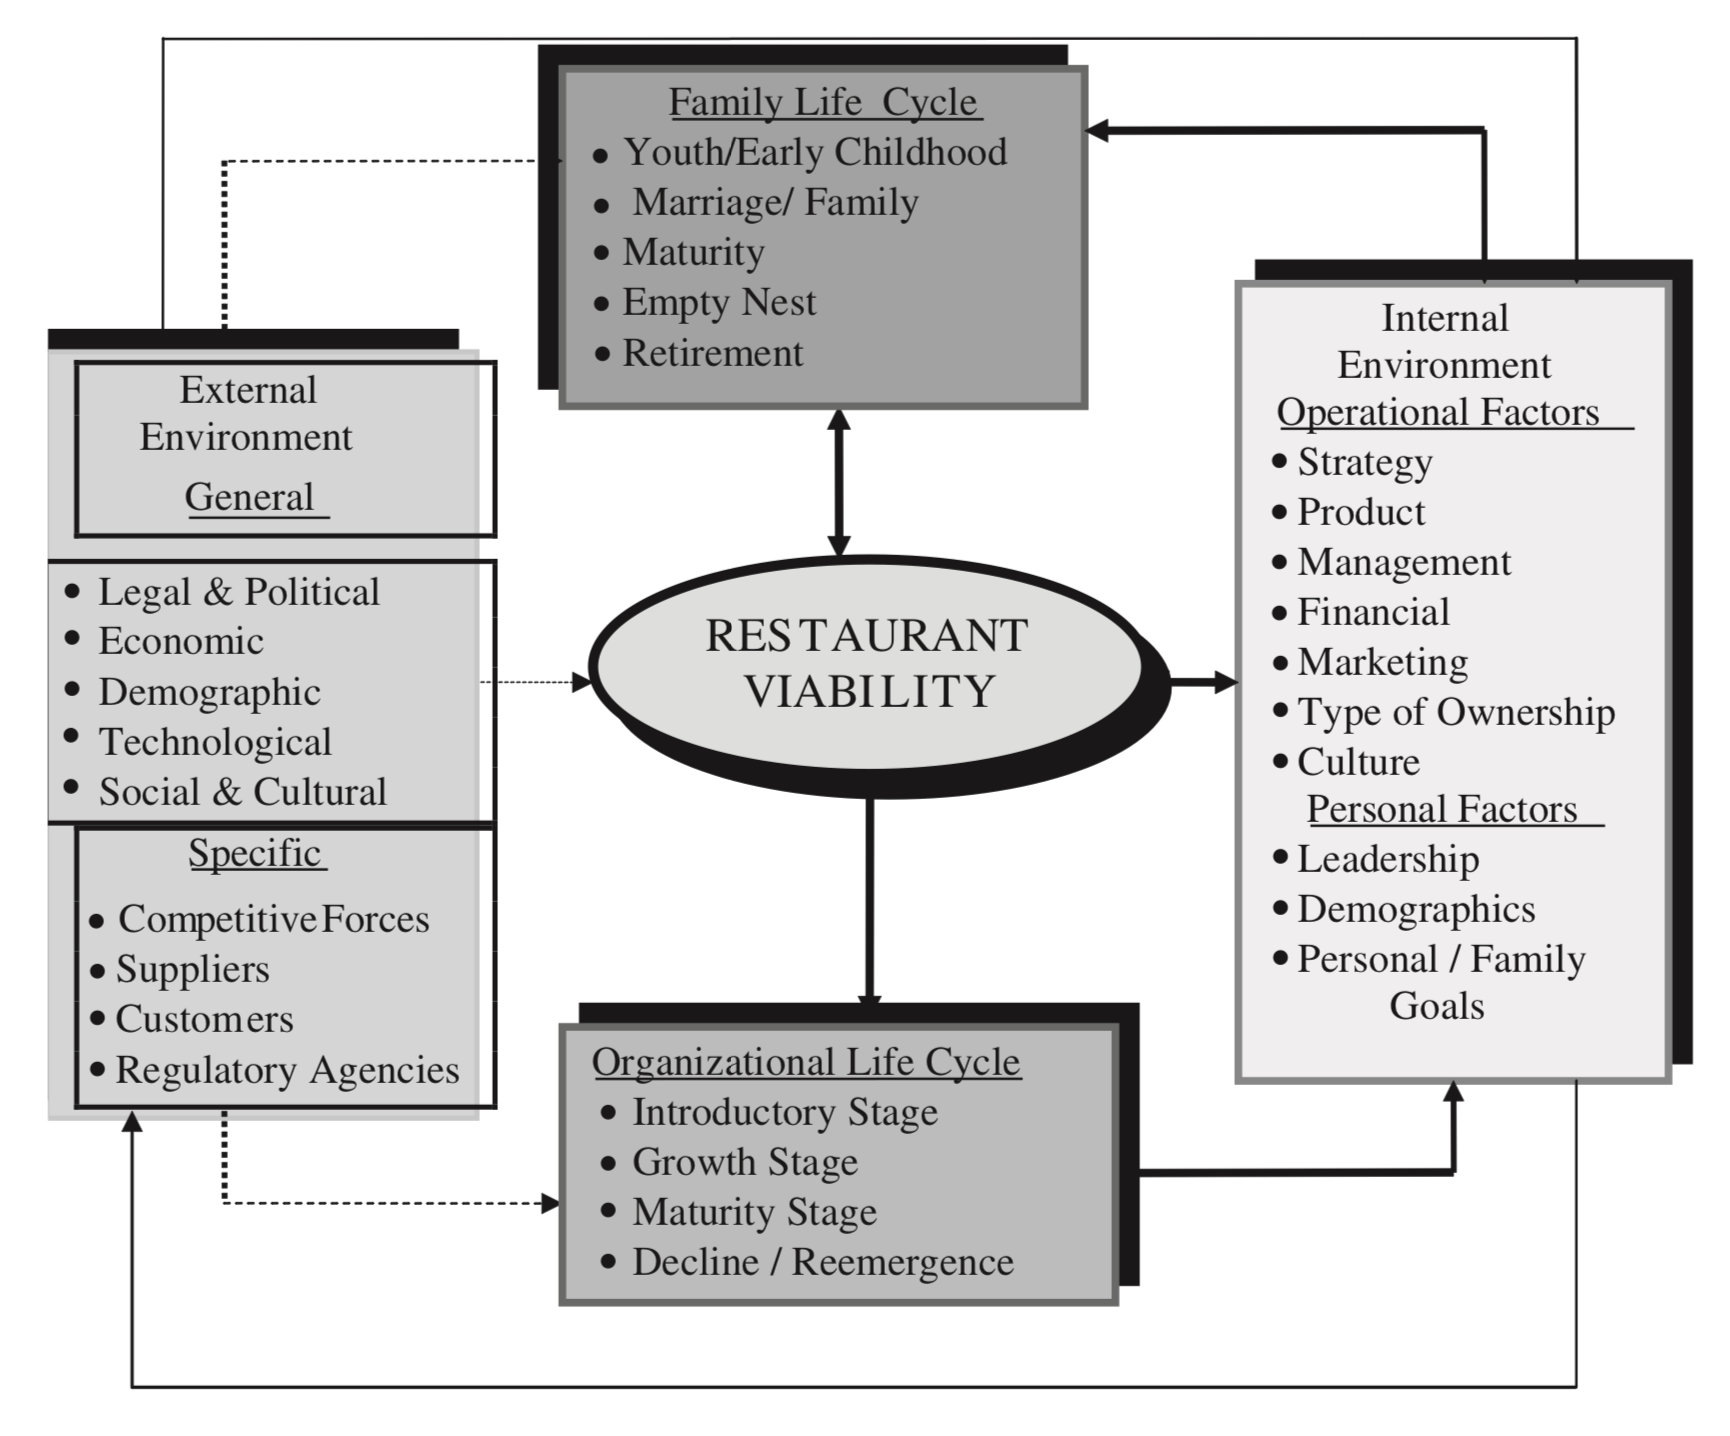
\includegraphics[scale=0.5]{Figures/Restaurant_sucess_factors/Factors_on_restaurant_viability.png}
\centering
\caption{Impact of various factors on restaurant viability \cite{Parsa.2005}}
\label{fig:Factors_on_restaurant_viability}
\end{figure}

For a successful restaurant, it is essential to secure a suitable location, maintain service levels and food quality, control the cost of labor, food and beverages, well-defined goals, finance, and marketing management, and strong leadership \cite{Parsa.2005}. The restaurant may fail or succeed due to any of these factors. A restaurant location has a significant impact on the success or failure of a restaurant , for example opening a nightclub restaurant near a police station thinking of safety may be a wrong selection of location as many customers will not feel comfortable due to police scrutiny. This project aims at selecting a prospective site for a new restaurant while considering location-dependent features which may impact restaurant success.

\section{Elements of a restaurant location analysis}
\label{elements}


The location of a restaurant plays a critical role in the success or failure of a restaurant business \cite{Parsa.2005} \cite{Tzeng.2002} \cite{Camillo.2008}. Not every place may be a suitable location for every kind of restaurant. There are various factors such as demographic values of the restaurant neighborhood, accessibility, visibility, and others, which need to be taken into account when selecting the location for opening a new restaurant. Location analysis techniques are applicable to find the best place for a new restaurant. Some of the elements of restaurant analysis techniques are \cite{EvanTarver.21.04.2017} \cite{Webstaurantstore.com.25.07.2018}:


 \textbf{1.	Demographics}

Demographics information of the neighboring population such as age, gender, income, religion, relationship status, environment, and ethnicity have an decisive effect for potential restaurant owners on choosing a restaurant category like “fast food”, “casual dining”, “fine dining” or “bar \& bistro” \cite{EvanTarver.21.04.2017}. For example, fast food restaurants are often favored by people with demographic criteria such as an age range between 15 and 35, often pedestrians with a low income. The visit to fast food restaurants is usually unplanned and connected to other nearby events like shopping. Fine dining restaurants, in contrast, are favored by people older than 35, couples, high-income people, as pre-planned activities and usually mostly by vehicle traffic.

\textbf{2.	Psychographics}

Psychographics information such as personality types and personal preferences of consumers support the decision of cuisine types \cite{EvanTarver.21.04.2017}. For example, family-oriented and tradition-oriented consumers usually prefer Italian restaurants, whereas health-conscious consumers regularly choose organic or vegan grill restaurant. 

\textbf{3.	Population}

Information about the people and the population density in a specific area are necessary to launch any new business or product as defined by the \ac{cpt} \cite{Chen.2016}. A location must fulfill the criteria of \ac{cpt} like range and threshold to be a viable location for new business launch. The range quantifies the maximum distance that consumers travel for a desired meal and threshold is the minimum population required around the site to start a business or product (restaurant).

\textbf{4.	Customer Activity: Foot \& Vehicle Traffic}

For a location to be successful, it should have high levels of activities of potential customers around it, like in the neighborhood of downtown and tourist places \cite{EvanTarver.21.04.2017}. Foot traffic increases the flow of potential customer walking by a restaurant, whereas vehicle traffic enhances the information to customers who would potentially drive to the restaurant.


\textbf{5.	Competitor Analysis}

Analyzing the competitors that are already active in an area can be beneficial in multiple ways \cite{EvanTarver.21.04.2017}. If a location has too many restaurants in the neighborhood, on the one side this means that the regional market is healthy and supportive in that area and the chances of success are high in that area. However, on the other side, it may be difficult to enter the market and attract customers due to the competition, so sometimes it is better to find a location with less competition, but in which demand still exists. 

\textbf{6.	Labor Cost \& Minimum Wage}

Restaurant environment effects such as the cost of labor, minimum wage and the availability of potential employees vary with different locations \cite{Webstaurantstore.com.25.07.2018}. These factors influence the profit and success of businesses to a large extent. Therefore, these pieces of information must be collected and taken into consideration before choosing the location for a restaurant.

\textbf{7.	Accessibility and Visibility}

For a position to be a potential spot for the opening of a restaurant, it should be easily accessible by foot traffic and car traffic with accessibility to nearby parking area \cite{Webstaurantstore.com.25.07.2018}. Moreover, it should not be in a place where the traffic is too high, and the restaurant would not be visible by drivers or pedestrians.

\textbf{8.	Proximity to suppliers}

Proximity to suppliers is critical, as shipping cost and delivery cost of supplies might be higher than the original net procurement costs of goods if it not chosen wisely \cite{Webstaurantstore.com.25.07.2018}. The optimal choice of a location should minimize these expenses for the business to be successful.

\textbf{9.	Crime Rates}

A potential restaurant location should only be finalized after researching in detail about the crime rate and the type of crime in the respective area \cite{Webstaurantstore.com.25.07.2018}. Consumers generally do not prefer eating out in areas with high crime rates, and it may be a significant factor leading to the failure of a business. 

\textbf{10.	Future Growth}

Future restaurant owners should consider plans and aspirations in the choice of restaurant locations \cite{Webstaurantstore.com.25.07.2018}. In the case that the restaurant prospers and gains popularity, it may require an increase in the customer and employee capacity. Moreover, there should be sufficient parking spaces and storage options.

\textbf{11.	Health regulation and zoning}

Different parts of cities have different rules related to health and zones only allowed to certain types of businesses \cite{Webstaurantstore.com.25.07.2018}. These regulations should be reviewed and appropriately researched before finalizing the location. 




\chapter{Data sources}
\label{Data sources}
\lhead{\emph{Data sources}}

As data is an essential requirement of projects based on machine learning, this chapter discusses the different sources which provide data relevant to the project.

\section{Transparency Portal Hamburg}
As the first German federal state, Hamburg enacted a transparency law on October 6, 2012 \cite{Murjahn.2016}. Opposed to a right to request information, which all citizens had until this date, a new duty to inform the public was laid upon the state’s administration offices. All information that would fall under this law now had to be published in a freely available standard format on centered storage of data. The single pieces of information, which would fall under the law, varied highly in precision and the comprehensive term of ``geodata'' was requested opposed to precise datasets of geodata. A legal interpretation was worked out for all essential points, and a plan for the release of geodata was designed consisting of the underlying data for measurement administration and the technical geodata for special administration offices. The transparency law granted a period of two years for technical implementation.

In October 2014, the ``Transparency Portal'' (http://transparenz.hamburg.de/) as the major component of the implementation of the transparency law was released \cite{Murjahn.2016}. With this portal, the Hamburg citizens have a multitude of data and documents available that was prior only available to Hamburg's administration. One important focus was the release of geodata that was even before the law in preparation for an ``Open GeoData'' model. In this ``Open GeoData'' model, geodata was split into two groups of data sets, one group able to be extracted with little effort, but free to the public and expected with high use, and another group with expected high demand and high revenue on the sale of this data. For this second group of datasets, more effort with new measurements had to be arranged. With the transparency law in place, all datasets were merged into the Transparency Portal and yielded a much higher download count than the count of dataset sales before the portal was active. The Transparency Portal uses a standardized metadata repository called the \ac{metaver} in collaboration with other German federal states.

\section{Online restaurant review portals}

As described in the introduction, the basis for the success of a restaurant in this paper is determined by the number of and rating of reviews in online restaurant review portals since these reviews are visible to the public and available for every restaurant on the portals. Review portals for restaurants provide a platform for users to discuss their experience in these businesses and thereby influence the decisions of other customers to visiting these restaurants \cite{Mellet.2014}. Review portals present a view of the success of restaurants, which both the restaurant owner as well as their potential customers see.

\subsection{Tripadvisor}

Tripadvisor is one of the biggest rating portals for travel and travel-related businesses, such as restaurants, with cumulated 600 million reviews and opinions until 2017 \cite{StephenKaufer.27.04.2018}. This made Tripadvisor a potential portal for the analysis of restaurant reviews to extract data from. However, it was found that any scraping, download or copy of the data with automated or manual methods is legally prohibited from Tripadvisor, which excluded Tripadvisor as a data basis for the analysis of this paper.

\subsection{Google Places}

As Google is the most frequently used search engine on the world and since the research of consumers on the internet before any buying decision increases, the data processing company Google may have a high influence on purchase decisions \cite{Zhao.2018} \cite{Shim.2001}. It further provides a service called ``Places'' for local businesses, among them restaurants, to present themselves with an opportunity of customers to leave reviews, ratings, and answers on common questions \cite{GooglePlaces}. With 100 million places, 25 million updates per day and one billion active users per month, the platform may provide insightful data to the restaurant landscape in Hamburg. The Places \ac{api} provides an interface for developers to receive data about places, thereof restaurants, that may be used for analysis. 

However, when the \ac{api} was explored more thoroughly, only the first five reviews of any restaurant could be retrieved, and the review count was not extractable. Without the review count, there was information, how well a restaurant had been rated, but not how many customers have rated it, which is essential information. Therefore, Google Places was discarded as a potential source of restaurant information for this paper.

\subsection{Facebook}

Social media is vital in the influence on customer choices of products, especially when customers prepare travel or plan the stay at a venue like a hotel or a restaurant \cite{Kwok.2013}. In these cases, online reviews are often taken into consideration. Companies in the hospitality sector, therefore, have to aim at the benefits of social media tools carefully. Facebook, as one social media platform, has a large customer base with 2.32 billion monthly active users in the fourth quarter of 2018 \cite{statista.facebook.2019}. Out of these reasons, Facebook was considered as one portal to analyze restaurant data from. The Facebook Graph \ac{api} provides access to content on Facebook for developers \cite{facebook.graph.2019}. This Graph \ac{api} is designed for apps that can read and write to Facebook and thereby connects a third-party service with Facebook.

Despite Facebook being a potential source of information of publicly visible restaurant data, the access to this information was impeded by an app review process. In May 2018, Facebook launched an enhanced developer app review, which made it necessary for developers to verify one's business, sign a supplemental terms contract and provide means of proving the business, such as utility bills or taxi ID numbers \cite{KonstantinosPapamiltiadis.01.05.2018}. Since this was not available and since there was no intention of creating a business app on Facebook, Facebook as a source of restaurant information was discarded for this paper.

\subsection{Yelp}

Yelp is a popular and widely used social networking site for reviewing and sharing information about local businesses like restaurants, dentists and mechanics \cite{YelpInc..2018}. Yelp was founded in 2004 in San Francisco, California, and currently operates in 32 countries. It had an average of 164 million unique visitors every month (via the Yelp app, mobile web, and desktop) and had 177 million reviews in 2018. Moreover, it presents information about events, special offers and provides a platform to connect and discuss among yelpers (registered users on Yelp). The company Yelp Inc. sells advertisements to local businesses, but they claim that reviews do not get affected by advisements, e.g., in the form of added, manipulated, deleted comments. Figure \ref{fig:yelp_factsheet_figures} shows the statistics for the distribution of user ratings, recommendations, and businesses reviewed by category for review across all categories as of 31st December 2018 \cite{YelpInc..2018}.

\begin{figure}[h]
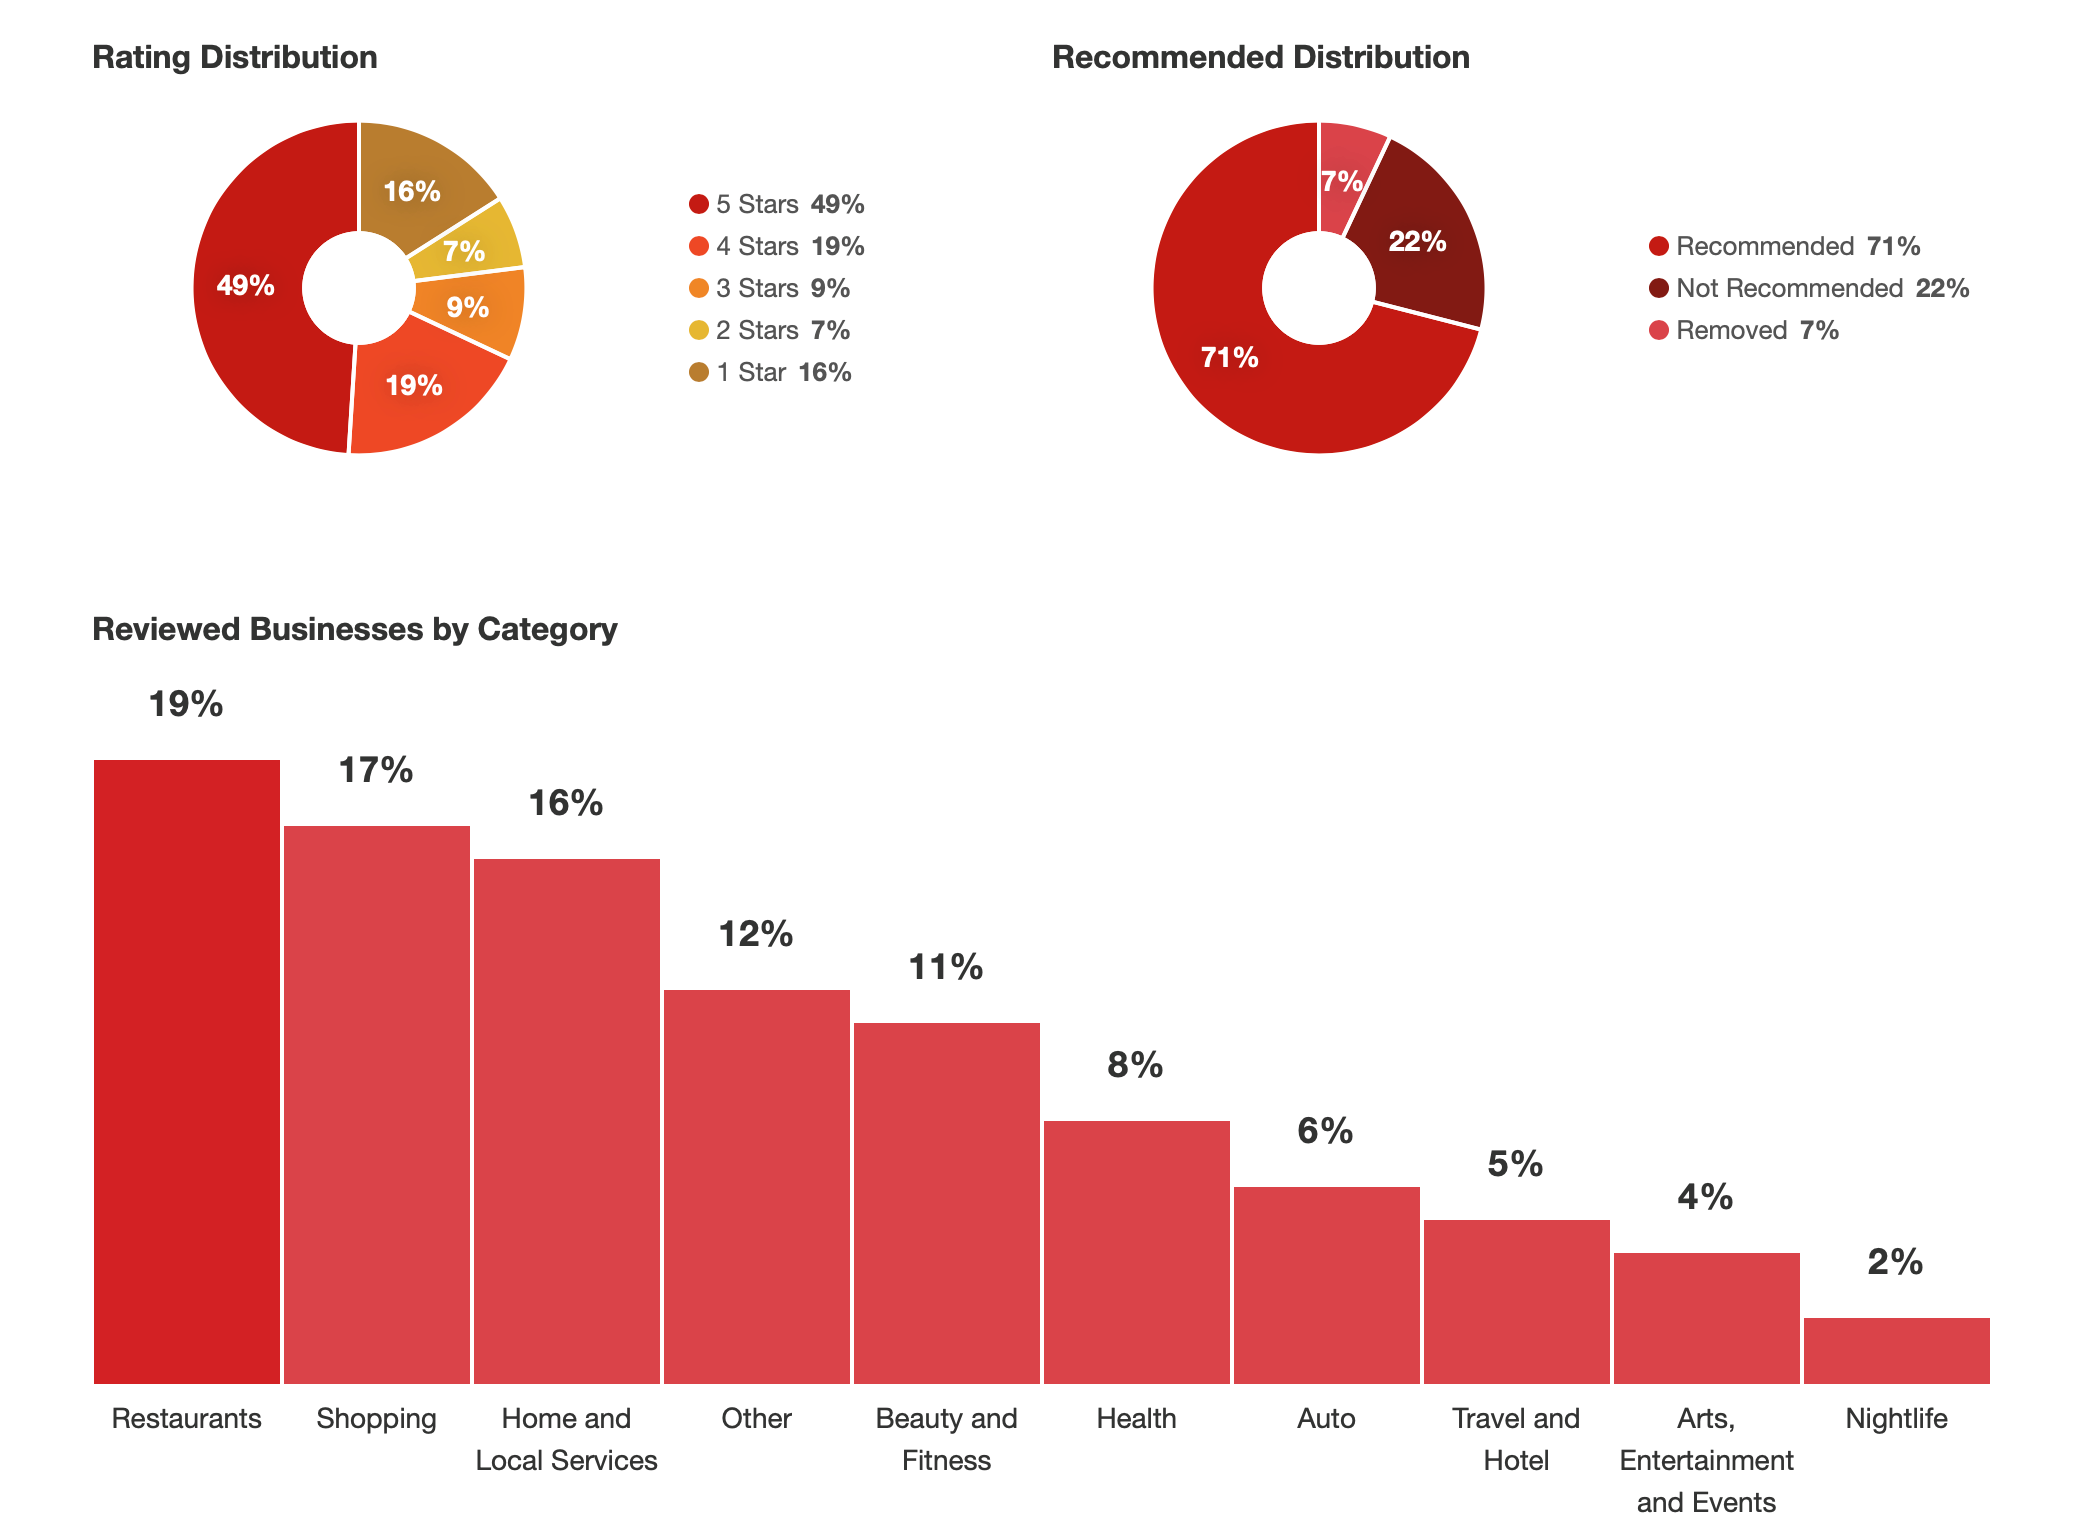
\includegraphics[scale=0.5]{Figures/Yelp_Factsheet_Figures.png}
\centering
\caption{Statistics on Yelp review according to Yelp Inc. \cite{YelpInc..2018}}
\label{fig:yelp_factsheet_figures}
\end{figure}

From Figure \ref{fig:yelp_factsheet_figures}, it can be seen that the restaurants had the maximum of reviews among all categories and the rating distribution and recommended distribution shows that yelpers use Yelp to share positive as well as negative experiences. The general, different types of information Yelp collects about restaurant businesses are ratings, reviews, price categories (inexpensive, medium, high, ultra-high), neighborhood, parking facilities, type of meal served (breakfast, brunch, lunch, dinner), smoking areas, reservation possibilities, delivery services and adequacy for children or groups, etc. \cite{YelpInc..2018}.  


 
 \chapter{Analysis methods}
 \label{Analysis_methods}
\lhead{\emph{Analysis methods}}

The chapter discusses the methods used for the location success prediction and the measures used to verify the predictions’ accuracy.

\section{Random Forest Regression}
\label{sec:random_forest_regression}

\ac{rfr} is a supervised regression machine learning technique that applies an ensemble learning method \cite{Gromping.2009}. It is used as the main regression technique for restaurant success prediction based on a location in this paper and is described in this section.

\subsection{General description}

The \ac{rfr} builds so-called “random forests”, which are groups of multiple decision trees per random forest \cite{Gromping.2009}. Predicted regression values of \ac{rfr}s are an average of prediction values from each of the trees that they comprise. The term “random” stems from the fact that individual trees only use a random subset of the observations and the tree splits within a tree as well is based on a random subset of variables. Building these random subsets of observations and attributes, each creating another tree, is conducted in a defined number of iterations. The use of random feature subsets in the \ac{rfr} technique makes \ac{rfr} predictions more robust against overfitting than in other techniques, such as support vector machine and neural networks \cite{Liaw.2002}. Moreover, \ac{rfr} has been found to deliver more accurate predictions in cases, in which the number of variables is higher than the number of observations. In addition, \ac{rfr} provides two important pieces of information:

\begin{enumerate}
\item	 Variable importance: \ac{rfr} can measure the contribution of variables to predictions \cite{Liaw.2002}. The measure of variable importance can be used to prune less important variables since the likelihood of overfitting increases with the number of variables.
\item Proximity measure: Proximity measures the closeness of data points to each other and a proximity matrix can be generated \cite{Liaw.2002}. The proximity matrix may then be used to study structure in the data.
\end{enumerate}

\subsection{Random Forest Regression Algorithm}

The steps in the algorithm of \ac{rfr} can be described as follows \cite{Liaw.2002}:

\begin{enumerate}
\item	From a given dataset, a defined number of bootstrap samples for trees is drawn.
\item Unpruned regression decision trees for each of the bootstrap samples are developed. Individual trees are based on random subsets of the observations and the splits within the trees are based on random subsets of variables after the defined number of iterations.
\item The dependent variable is predicted for new feature sets by calculating the average of the tree prediction.
\end{enumerate}

\subsection{Estimation of the random forest error rate}
An estimation of the error rate in \ac{rfr} is obtained with the help of the training data by conducting the following steps \cite{Liaw.2002}:

\begin{enumerate}
\item Available data outside of the bootstrap sample (\ac{oob} data) is predicted at each iteration of bootstrapping.
\item The error rate is calculated by aggregating the \ac{oob} predictions. The result of this is known as the \ac{oob} estimate of error rate.
\end{enumerate}
 
\subsection{Bagging and boosting}

Bagging and Boosting are two techniques to construct an ensemble of individual classifiers (trees) \cite{Dietterich.2000}. Individual trees of an ensemble are diverse, and higher accuracy of predictions can be obtained by the aggregation and voting of the results of single trees. In the bagging technique, each training set is constructed by replicating the bootstrap sample of the original training set. The single bootstrap samples in this process are called “examples”. The example creation in the bagging technique is conducted in parallel. In this process, a defined number of examples are taken from a given training set from the entire population of available data. These examples form a new training set. Multiple of these subsets of the training set are created to build multiple trees in the ensemble. Boosting techniques, in contrast, are based on assigning weights to the original training set and adjusting these weights after each regressor prediction. Boosting is a sequential process, in which weights are increased for the examples which are mispredicted and decreased for correct predictions. Moreover, the predictions are less affected by noise in bagging than in boosting. Additionally, bagging constructs several trees, only if small variations in the training set cause a large variation in the prediction outputs. \ac{rfr} uses the bagging technique in combination with techniques to randomize the internal decisions of the learning algorithm to create several regression trees.


\section{Regression performance measures}
\label{sec:Regression performance measures}

A common performance measure for the quality of fit of regression models is the ``coefficient of determination'', which is also called ``$R^2$'' \cite{Devasthali.2018}. This coefficient of determination uses a baseline model, which is a model that consistently predicts the mean of all observations of the dependent variable. This baseline model is a model that a created regression model can be compared to, to see how much more accurate the own predictions were to a poor model.

Following are the calculation of the \ac{sse}, \ac{sst} and $R^2$ \cite{Devasthali.2018}:

\[SSE = \sum\limits_{i=1}^n (y_{i} - \hat{y}_{i})^2\]

\[SST = \sum\limits_{i=1}^n (y_{i} - \hat{y}_{i})^2\]

\[ R^2 = 1 - \frac{SSE}{SST}\]

According to this calculation, $R^2$ always lies between 0 and 1, if the created regression model yields more accurate predictions than the baseline model \cite{Devasthali.2018}. The closer $R^2$ is to 1, the closer are the predictions by the regression model to the actual values. Additionally, the higher $R^2$ is, the more variations of the dependent variable are explained by the model.

A weak point of $R^2$ is that additions of more independent variables never lower the value of $R^2$, even for variables with little or no information gain \cite{Devasthali.2018}. To cope with this problem, another performance measure called ``Adjusted $R^2$'' was introduced, which introduces a negative effect on the measure for the inclusion of ineffective variables. It is calculated as follows \cite{Devasthali.2018}:

\[ \bar{R}^2 = 1 - (1-R^2)\frac{n-1}{n-p-1}\]

n = no of data points

p = no of independent variables in the model

$R^2$ therefore only improves (moves closer to 1), if significant variables are added to the model, and deteriorates (moves closer to 0) if variables are added that are not valuable to the prediction of the dependent variable \cite{Devasthali.2018}. 

\chapter{Data extraction}
\label{Data extraction}
\lhead{\emph{Data extraction}}

The extraction of data from the various sources was carried out using different techniques which this chapter describes in detail.

\section{Hamburg district map}

Since cities usually raise important figures in aggregation per administrative area, in Hamburg being the single city districts, these administrative areas should be imported into QGIS to be able to link single restaurants to an administrative area and hence figures that could be important as dependent variables to predict restaurant success. The borders of the administrative areas are taken from a dataset of the Transparency Portal called ``ALKIS Verwaltungsgrenzen Hamburg'' \cite{LandesbetriebGeoinformationundVermessung.28.02.2018}. This dataset is available in multiple data formats, is reported to have a 0\% data deficit and a precision of 0.1 meters. It is part of the \ac{alkis}, a digital combination of the real estate book information and a real estate map \cite{ALKIS2019}.

For this analysis, the \ac{gml} version of the administrative boundaries was downloaded and imported to QGIS. Loading the administrative boundaries into QGIS, the \ac{etrs89} \ac{crs} defined by EPSG:25832 was selected, as was defined in the metadata of the dataset. All following elements that are loaded into QGIS are as well projected in this \ac{crs}. The imported boundaries can be seen in figure \ref{fig:administrative_boundaries}.

\begin{figure}[h]
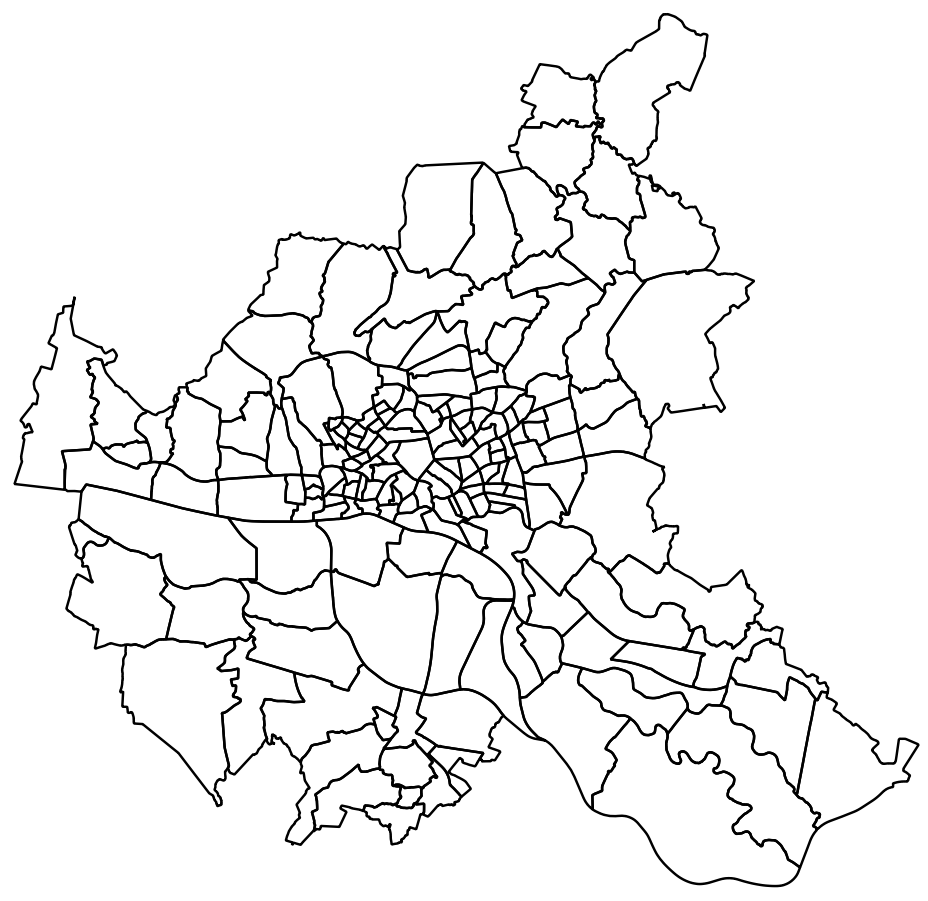
\includegraphics[scale=0.5]{Figures/Hamburg_Administrative_Boundaries.png}
\centering
\caption{Administrative boundaries of Hamburg in QGIS}
\label{fig:administrative_boundaries}
\end{figure}


\section{Yelp restaurant data extraction}

Yelp provides developers with an \ac{api} called Yelp Fusion \ac{api} for accessing the Yelp database. The authentication of \ac{api} calls is done via a private \ac{api} key which can be obtained by:
\begin{itemize}
\item Registering for a Yelp developer account, and
\item Creating an application
\end{itemize}

An extensive guide on the Yelp API authentication is provided on Yelp’s documentation page \cite{Yelp.Fusion.Authentication}.
For this project, \ac{api} calls were conducted using Python 3.7.

\subsection{Raw data extraction}

The extraction of data from the Yelp database consists of the following two steps, which are described in detail in this section:
\begin{enumerate}
\item Loading raw data by performing search queries using Yelp’s Python \ac{api}
\item Wrangling data into intermediate formats and storing wrangled data for further analyses
\end{enumerate}

\subsubsection{Retrieving data within a specific area from the Yelp server}
\label{retrieving_data_within_a_certain_area}

The yelpapi Python module \cite{GeoffreyFairchild.11.07.2018} must be installed in Python to perform \ac{api} calls. The obtained private \ac{api} key must be stored as a Python string:

\begin{verbatim}
from yelpapi import YelpAPI
api_key = ‘pastetheapikeyhere’
yelp_api = YelpAPI(key)
\end{verbatim}

Each search query is an https request to the Yelp server. The Python Yelp API exposes this as the following function:
\begin{verbatim}
yelp_api.search_query()
\end{verbatim}

The list of parameters for this function is the same as the https query which is provided by Yelp \cite{yelp.businesses.search}. For this project, this function was used as:
\begin{verbatim}
response = yelp_api.search_query(term='restaurants',
	 	latitude=latitude, longitude=longitude, 
		limit=50, offset=0, radius = radius)
\end{verbatim}
where latitude, longitude and radius defined the centroid of the search area.
Note that for each query, only a maximum of 50 restaurants could be returned (default=20). This means that:
\begin{itemize}
\item The total number of restaurants had to be extracted from the returned object of the first function call
\item The function had to be called multiple times to get data for all the restaurants within the desired search area
\end{itemize}
This process was built into the get\_restaurants(latitude, longitude, radius) function in the Python file yelp\_hamburg\_load.py.

\subsubsection{Determining latitudes and longitudes for restaurant searches}
\label{Determining_latitudes_and_longitudes_for_restaurant_searches}

To receive data from all restaurants in Hamburg, the city had to be divided into tiles of size 2,000 meters by 2,000 meters. As Yelp only responded with less or equal than 1,000 restaurants, the tiles were even quartered, when precisely these 1,000 restaurants were sent back, in the Python scripts ``analysis\_big\_tiles.py'' and ``get\_big\_tiles.py''. With smaller tiles, all restaurants could be retrieved. The vertices of the tiles were the latitudes and longitudes used by the function get\_restaurants() mentioned in section \ref{retrieving_data_within_a_certain_area}. This process consisted of the following steps:
\begin{itemize}
\item Pre-determine the maximum latitude, maximum longitude, minimum latitude and minimum longitude of Hamburg. These points were manually picked out from a map of Hamburg in QGIS.
\item Create a new empty list of latitudes and a new empty list of longitudes.
\item Inner loop: loop from the minimum longitude to the maximum longitude, incrementing by 2,000 meters (length of tile’s side). Append each new longitude into the list of longitudes.
\item Outer loop: loop from the minimum latitude to the maximum latitude, incrementing by 2,000 meters (length of tile’s side). Append each latitude into the list of latitudes.
\end{itemize}

Note that the set of pre-determined maximum/minimum latitudes and longitudes were of \ac{etrs89} (EPSG:25832) \ac{crs}, while Yelp \ac{api} calls require WGS84 (EPSG:4326). Therefore, a helper function [transform\_coord()] using the Python module pyproj \cite{JeffWhitaker.2018} was written to transform the formats of the latitudes and longitudes so that they could adequately be passed into the Yelp \ac{api} calls.

\subsubsection{Extracting data of restaurants in Hamburg}
\label{Extracting data of restaurants in Hamburg}
As mentioned in section \ref{Determining_latitudes_and_longitudes_for_restaurant_searches}, each Yelp search query requires a latitude, longitude, and radius to determine the search location.

The radius of each search was calculated by the radius of all overlapping circles that could form a complete grid as shown in figure \ref{fig:Yelp_extraction_grid}. To receive all restaurants in a grid of tiles having a square of 2,000 meters by 2,000 meters, the radius of the searches needed to at least contain these squares. The longest distance of a square center to any point in the square is given by the distance of the square center to the edges. This distance can be calculated with the law of Pythagoras. If `c' is the distance of a triangle with `a' being the distance of the center of the square to the center of the left side of the square and `b' being the distance from the center of the left side of the square to the top left corner, then

\begin{equation}
 a^2 + b^2 = c^2
\end{equation}
 
\begin{equation}
 c = \sqrt{a^2+b^2}
\end{equation}
 
\begin{equation}
 radius = \sqrt{Tile Size/2 + Tile Size/2}
\end{equation}
The corresponding code for the calculation of the radius was given by the following formula:

\begin{verbatim}
radius = int(math.sqrt(math.pow(TILE_SIZE,2)*2))
\end{verbatim}

which was constant during all Yelp \ac{api} calls.

\begin{figure}[h]
\includegraphics[scale=0.4]{Figures/Yelp_extraction_grid.jpeg}
\centering
\caption{Yelp data extraction search grid}
\label{fig:Yelp_extraction_grid}
\end{figure}

Each \{latitude, longitude\} pair to be passed into each Yelp API calls was taken from the lists of latitudes and longitudes created in section \ref{Determining_latitudes_and_longitudes_for_restaurant_searches}.

The function get\_restaurants(latitude, longitude, radius) was called for each \{latitude, longitude\} pair until all pair combinations were used.

The result of each call was stored into a \ac{json} file respective to the latitude and longitude used with the help of the Python \ac{json} \cite{json.encoder} module. All generated \ac{json} files were subsequently merged into one \ac{json} file for ease of data wrangling.

\subsection{Data wrangling and storing}

As data in the \ac{json} file mentioned in section \ref{Extracting data of restaurants in Hamburg} was split, it had to be loaded back into Python for processing by:
\begin{verbatim}
with open('merged_extract.json') as json_data:
  businesses = json.load(json_data)
\end{verbatim}

A namedtuple ``Restaurant'' was created as an object model into which data from the \ac{json} file would be passed. The data fields for this namedtuple reflects the data retrieved for each restaurant from the search queries. The namedtuple’s data fields include:
\begin{itemize}
\item epsg25832\_latitude
\item epsg25832\_longitude
\item epsg4326\_latitude
\item epsg4326\_longitude
\item price rating
\item review\_count
\item is\_closed
\item zip\_code
\item category\_restaurant\_id 
\item category\_alias
\item category\_title
\item category\_index
\end{itemize}

Initially, the data loaded from the \ac{json} file was a Python list of (nested) dictionaries. Therefore, data was un-wrangled using the dictionaries’ keys. For example, the `epsg4326\_latitude’ field for each instance of the namedtupple Restaurant would be:
\begin{verbatim}
epsg4326_latitude = biz['coordinates']['latitude'] 
\end{verbatim}
where ‘biz’ is a dictionary object representing data of one restaurant, which is part of the loaded list of dictionaries from the \ac{json} file.

\begin{figure}[h]
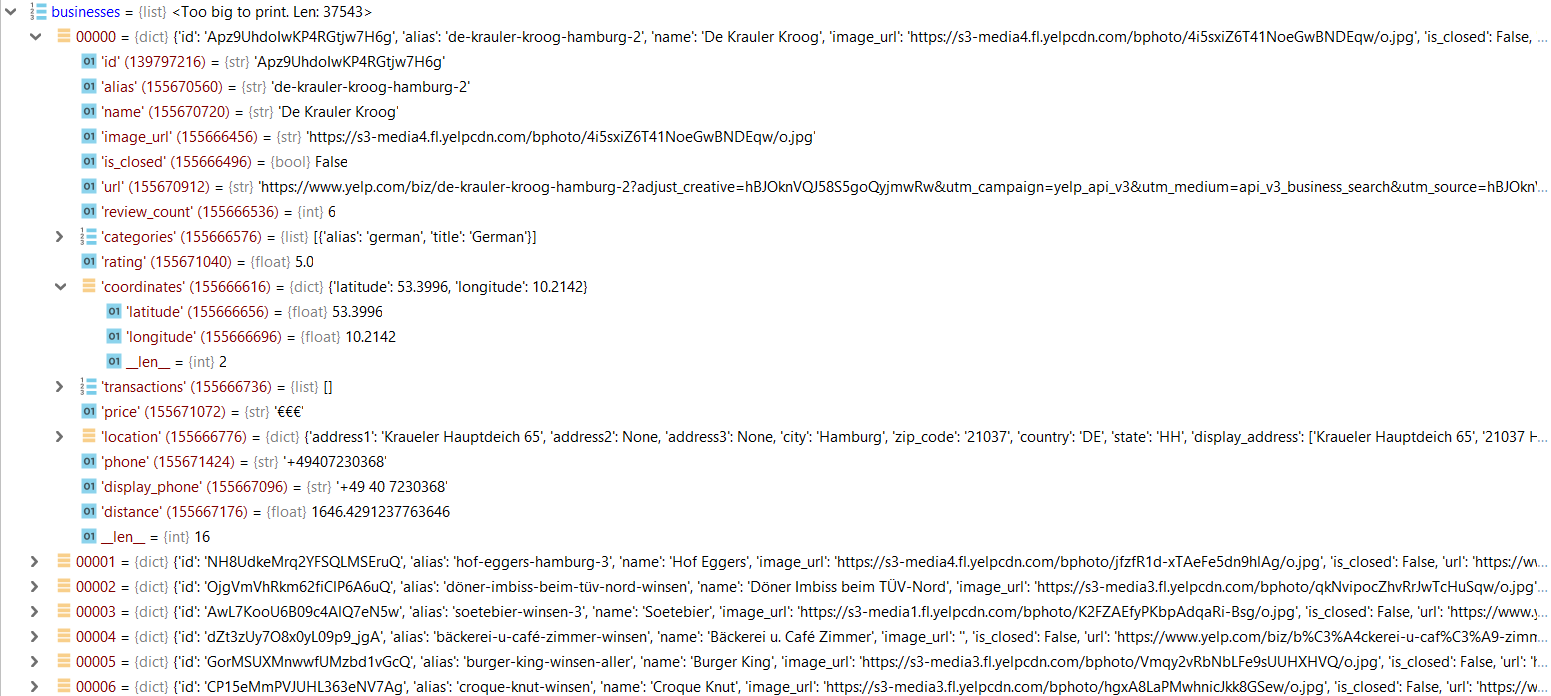
\includegraphics[scale=0.4]{Figures/restaurants_unwrangled.png}
\centering
\caption{Un-wrangled data from JSON file}
\label{fig:un-wrangled data from JSON file}
\end{figure}

\begin{figure}[h]
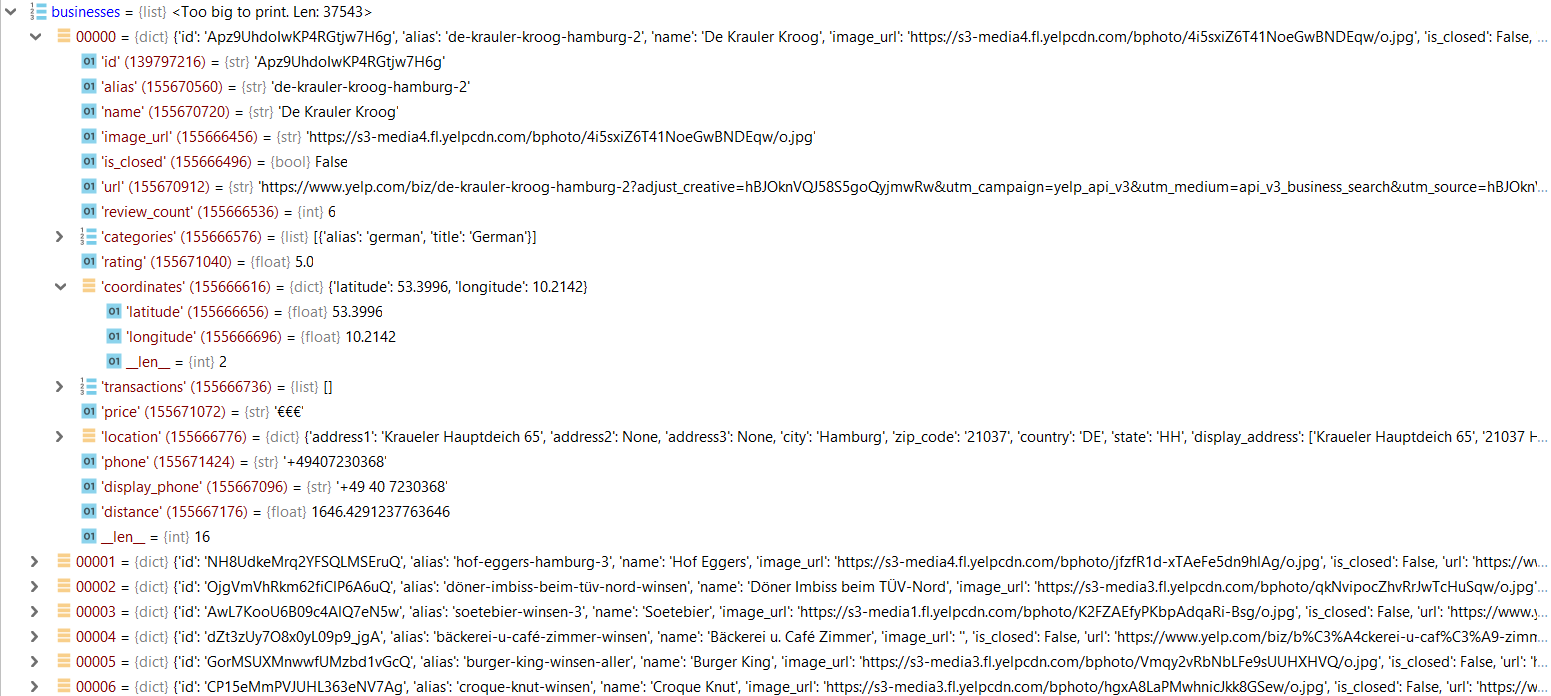
\includegraphics[scale=0.4]{Figures/restaurants_unwrangled.png}
\centering
\caption{Wrangled data stored in namedtuple}
\label{fig:wranged data stored in namedtuple}
\end{figure}

The list of namedtupples representing restaurants could then be passed into a pandas dataframes and subsequently stored into \ac{csv} files for further analysis.


\subsection{Restaurant success calculation}

The success of a restaurant is usually measured by financial figures, such as revenue, profit or business growth. However, this information is not publicly available for all small businesses, so a restaurant success has to be assumed from other metrics. Other metrics are important to businesses today are online reviews and ratings. They may influence the success of a restaurant and as well may mirror a restaurant's success. The rating and reviews a restaurant displays on a portal such as Yelp are their display of success to their customers on the Internet, for which reason the success measures in this paper should combine the two figures of review count and average rating.

In a Python script called ``add\_restaurant\_success.py'', the average rating and review count have been standardized to set them to a comparable range of values while still keeping the effects of outliers. The standardization has been conducted with the StandardScaler function of the scikitlearn-preprocessing package. Having the average rating and review count in comparable ranges, the values were added and saved into a success variable to value them equally in their part of the success. The success, hence, is the sum of the standardized Yelp review count and average rating. In figure \ref{fig:restaurant_success_distribution}, the distribution of the success values can be seen, they are in the range between ca. -4.2 and ca. 13.3.

\begin{figure}[h]
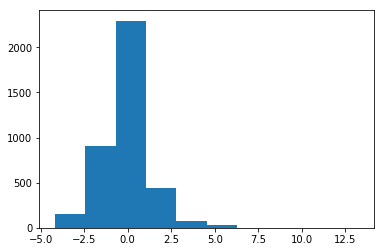
\includegraphics[scale=0.5]{Figures/restaurant_success_distribution.png}
\centering
\caption{Distribution of Restaurant Success Values}
\label{fig:restaurant_success_distribution}
\end{figure}


\section{City district profiles Hamburg}
\label{district_profiles}

In this study, it was considered that the city district that a restaurant was located in, may influence the success of this restaurant, e.g., through direct or indirect effects from the demographics in this district. Therefore, ``city part profiles'' published in the Transparency Portal of Hamburg were taken into account \cite{Profiles2018}. The dataset presents structure data for all of Hamburg's city parts for the topic areas of population, living, council elections, social structure, infrastructure, and traffic. The last dataset was published on the 19.03.2018, but dated back to data from 2016.

The data was available in XLSX-format, in which it was downloaded. Afterward, the formatting was adjusted to be able to save the content as a \ac{csv}. With this \ac{csv}, all the necessary information, that would later be used in the analysis, was available as a spreadsheet that could be loaded into Python. In a Python script called ``profile\_translation.py'', all values of the city district profiles were translated from German to English.

\section{Proximity to water}
\label{proximity_to_water}

As Hamburg is a famous port city and almost 10\% of the city is covered by the harbor \cite{HamburgStadt2019}, water is an essential consideration in the analysis of restaurant success. To know the water locations in Hamburg is important because restaurants are regularly not placed on water (restaurant boats are not considered as potential location candidates for simplicity). Additionally, water may influence the success of a restaurant with customers who may like to sit with a water view. Out of these reasons, the locations of water in Hamburg should be made out, and the proximity of each restaurant to the next water location should be calculated.

For the extraction of water location, a geological ground map of Hamburg in the scale 1:5,000 \cite{GeologischeKarte2019} was added as a \ac{wms} layer into QGIS, as depicted in figure \ref{fig:geologische_karte}. The dark blue color on this \ac{wms} layer indicates that an area is on water ground, e.g., a river. Since the water spots on the \ac{wms} layer were not able to be processed as measurable points, yet, they had to be preprocessed before. 

\begin{figure}[h]
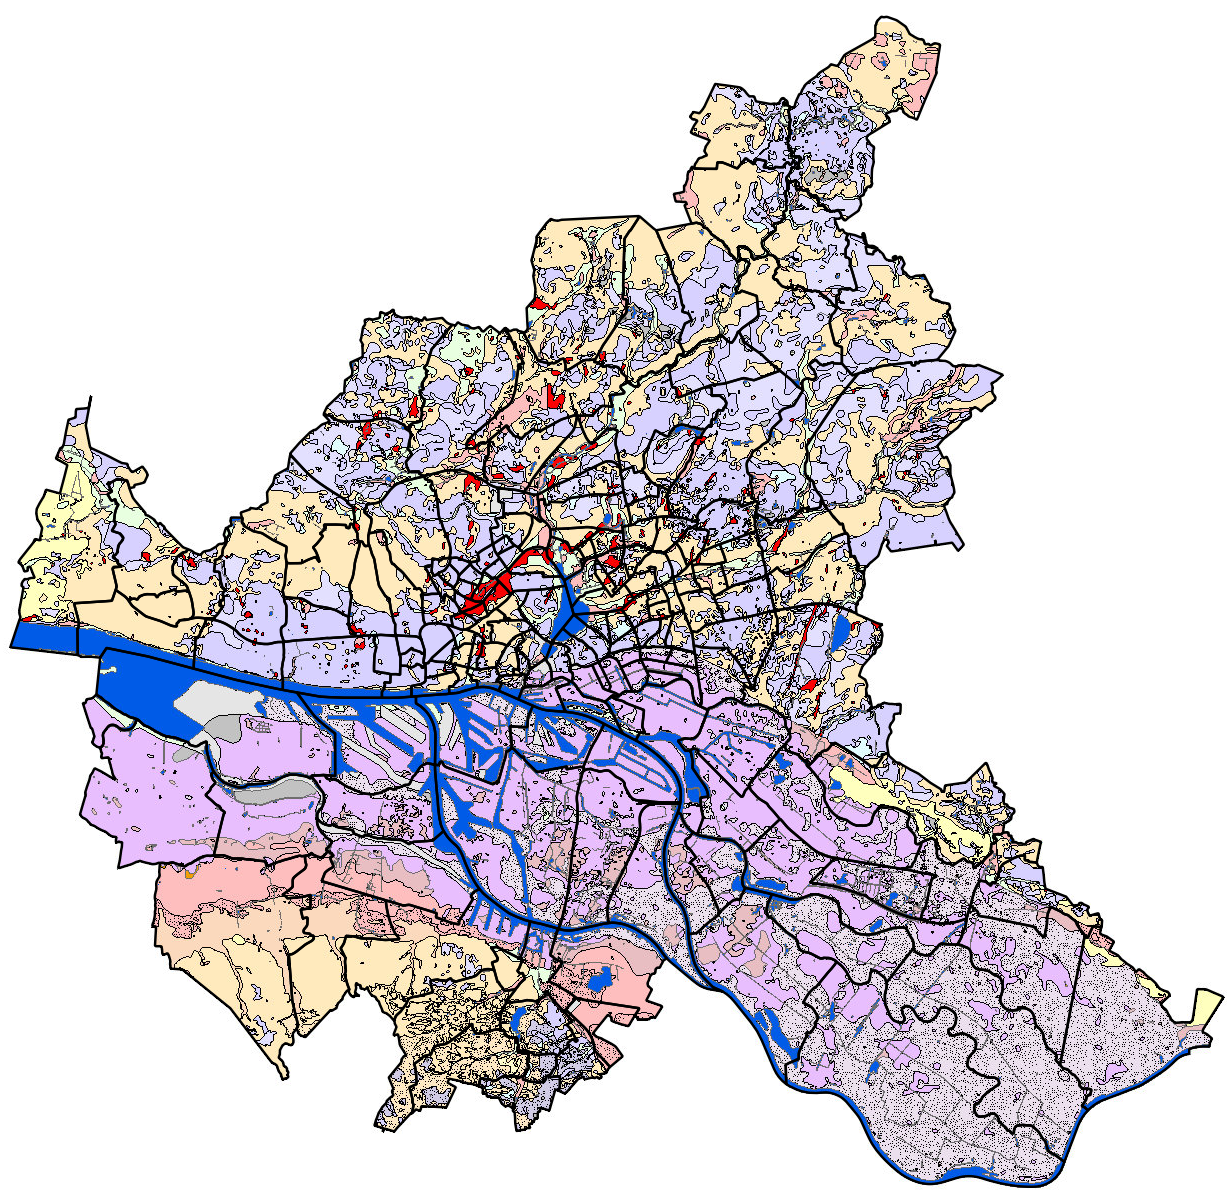
\includegraphics[scale=0.5]{Figures/WMS_Layer_Geologische_Karte.png}
\centering
\caption{WMS Layer ``Geologische Karte Hamburg''}
\label{fig:geologische_karte}
\end{figure}

In the first step, the \ac{wms} map was saved as a raster with the ``Save as...'' option of QGIS. The output was set to a ``Rendered Image'' in Format ``GTiff''. The \ac{crs} stays \ac{etrs89}, and the resolution is first set to 100\%. A new raster file is created.

The newly created raster file had a high resolution and needed to be reduced to be processed further. The resolution was reduced by conducting the QGIS raster conversion function ``Translate (Convert format)''. In the upcoming dialog, the ``outsize'' resolution was set to 3\%, and the output location was set to a new GeoTIFF file. In the created execution code in the bottom of the dialog, the standard ``of''-parameter ``GMT'' had to be changed to ``GTIFF''. The resolution was after the resolution reduction still adequate to present the water areas.

In the third step, the new and reduced raster file was converted into a grid that would store a particular color value for each of the points on the raster together with their coordinates. This could be conducted by using the same QGIS conversion function ``Translate (Convert format)'' as in the previous step, however, in the corresponding dialog, the ``outsize'' resolution was not touched, and the output format was set to an \ac{ascii} gridded XYZ file. In the generated XYZ-grid, three attributes per record could be found. The first two attributes present the x and y values on the \ac{etrs89} \ac{crs} and the third value a value for the colors with their luminosity is stored. The luminosity ``0'' is the darkest value in the grid and marks the prior dark blue water locations. This knowledge was used in a python script called ``extract\_water\_locations.py'' that was implemented to create a new dataset by looping through every record in the grid and keeping only the records, in which the luminosity would match ``0''. Thereby only water locations would be part of the new dataset.

The fourth step consisted of the calculation of the distances of each restaurant to the next water spot by using a Python script called ``calculate\_distance\_to\_water.py''. In this script, all restaurants and water locations were loaded into the memory. Then, for each restaurant, the lowest distance to water was calculated by looping through all water points and calculating the Euclidean distance to them. In the end, a minimum water distance was found for each restaurant that was stored together with the restaurant ID in a \ac{csv}-file for the use in analysis.

\section{Restaurant density}
\label{restaurant_density}

As described in chapter \ref{elements} on page \pageref{elements}, restaurant density is an important consideration in the selection of a location for a new restaurant. Therefore, this measure was included in the analysis of this paper. A pedestrian usually is willing to walk up to 400 meters to a nearby restaurant \cite{Yang.2012b}. Hence, the restaurant density would present the number of all restaurant, which would be in a range of 400 meters to a location. To include the restaurant density as a feature into the restaurant analysis, a Python script called ``get\_restaurant\_density.py'' was created, in which the Euclidean distance of all  restaurants to all other restaurants were calculated, and the ones with a proximity of 400 meters or less were counted to the density of a restaurant.

\section{Count of criminal cases}
\label{criminal_count}

The criminal activity near a location of a restaurant can be an important factor in the success of the restaurant, as explained in chapter \ref{elements}. The state office of criminal investigation in Hamburg uploaded a crime report in 2017, which presents different criminal activities per city district and additionally shows the total count of criminal activities per city district \cite{LandeskriminalamtHamburg.2017}. This total count of criminal activities was taken from the report and added as a record set for the analysis in the restaurant location analysis.

\chapter{Data analysis}
\lhead{\emph{Data analysis}}
\label{data_analysis}

Various attributes of the extracted dataset in this paper were analyzed for the use in a restaurant location analysis, and the predictions of multiple machine learning methods on the dataset were evaluated. In this chapter, these analyses and observations are discussed.

\section{Feature selection and preparation}
\label{sec:Feature_selection}

To prevent overfitting, the number of features in the training data should be kept to only the valuable features that support the prediction success in regression. The available data sources and features have been outlined in chapter \ref{Data extraction} on page \pageref{Data extraction}. 

Apart from the dependent variable represented by the calculated success of a restaurant, included restaurant information from Yelp are the price level of a restaurant represented by one or multiple Euro-signs, and the restaurant category, e.g., a café, Vietnamese restaurant or a Korean grill. To use these two pieces of information, they were discretized, and the restaurant category furthermore needed to be binarized. Additionally, with the location of a restaurant, the proximity to the next water spot and the restaurant density were calculated as explained in section \ref{proximity_to_water} and section \ref{restaurant_density} and added as features for the regressor training.

As explained in section \ref{district_profiles} and section \ref{criminal_count}, Hamburg provides city profiles with values representing each city district. Considering the factors for a restaurant location analysis explained in chapter \ref{elements}, the following attributes from the city district profiles were chosen to be included into the regressors training for a restaurant depending on the city district that the restaurant was located on:
\begin{itemize}
\item Count of criminal cases
\item Population
\item Share of under 18-year-olds
\item Share of foreigners
\item Population with migration background
\item Share of the population with migration background
\item Number of households
\item Share of one person households
\item Share of households with children
\item Share of households with single parents
\item Population density
\item Employment quote
\item Share of unemployed people
\item Sum of incomes per tax reliable person in EUR
\item Prices for properties
\item Prices for condominiums
\item Share of students in Gymnasium
\item Car density
\end{itemize}


The features were standardized to make the different value ranges of the several numbers comparable, .

\section{Regressor training}
\label{regressor_training}

In the training of a regressor, a regression technique is fitted to the training data to create a regressor that can predict values for unseen sets of feature values. In this paper, three different types of regression techniques were evaluated for their adequacy on the prediction of the restaurant success - \ac{rfr}, \ac{svr} and linear regression.

The available data was split into a training set containing 70\% of the data records and a test set containing 30\% of the training records. Each of the regressors was fitted with the training set and should then predict both the values from the training set as well as the values from the test set. All three steps of the train-test-split, regressor fitting, and prediction of test features were conducted 100 times to gain a more stable overview of the performance measures of the regressors. The $R^2$ and Adjusted $R^2$ values were measured for both the training and test predictions for all regressors and are explained in the following.

Based on experiences made with the training and test data, the \ac{rfr} regressor was set to consist of 1,000 trees and have a maximum depth of trees of five nodes. The \ac{svr} regressor was set to employ the \ac{rbf} kernel.

In figure \ref{fig:boxplot_r2_training_data} the $R^2$ values for the prediction of training set values for all three regression techniques are shown. It is visible that the random forest values vary between values of ca. 0.257 to 0.262, while \ac{svr} and \ac{lr} show $R^2$ values between ca. 0.23 than 0.24.

\begin{figure}[h]
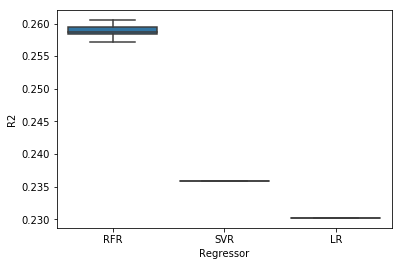
\includegraphics[scale=0.7]{Figures/Regressor_comparison/boxplot_r2_training_data.png}
\centering
\caption{Boxplot diagram of the $R^2$ values for training data predictions}
\label{fig:boxplot_r2_training_data}
\end{figure}

Figure \ref{fig:boxplot_adj_r2_training_data} presents the Adjusted $R^2$ values of the training data predictions of the regressors. While the Adjusted $R^2$  values of all three regressors are lower than their $R^2$ values (deviation of ca. 0.05 for each regressor) for the predictions of the same data, the order of regressors in their performance is the same. Hence, \ac{rfr} performs best on the training data among all three regressors.

\begin{figure}[h]
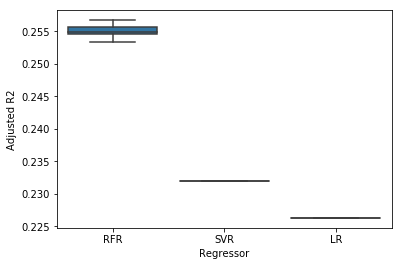
\includegraphics[scale=0.7]{Figures/Regressor_comparison/boxplot_adj_r2_training_data.png}
\centering
\caption{Boxplot diagram of the Adjusted $R^2$ values for training data predictions}
\label{fig:boxplot_adj_r2_training_data}
\end{figure}

The boxplot diagrams for the $R^2$ values of the test set predictions for all regressors are depicted in figure \ref{fig:boxplot_r2_test_data_all}. The \ac{lr} values are so low with values of $-4 * 10^{27}$ that the \ac{svr} and \ac{rfr} values are not displayed visibly. Therefore, the \ac{lr} values have been excluded in figure \ref{fig:boxplot_r2_test_data_without_lr}. It is recognizable that the \ac{svr} and \ac{rfr} predict the test values with much higher accuracy than linear regression and that \ac{svr} performs even slightly better than \ac{rfr}.

\begin{figure}[h]
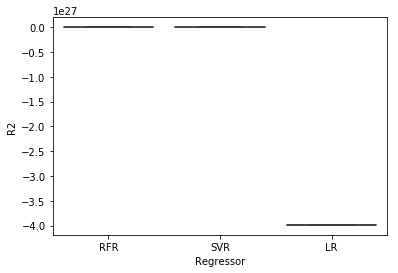
\includegraphics[scale=0.7]{Figures/Regressor_comparison/boxplot_r2_test_data_all.png}
\centering
\caption{Boxplot diagram of the $R^2$ values for test data predictions of all regressors}
\label{fig:boxplot_r2_test_data_all}
\end{figure}

\begin{figure}[h]
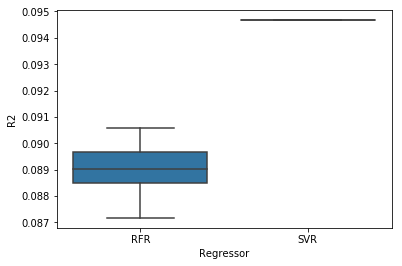
\includegraphics[scale=0.7]{Figures/Regressor_comparison/boxplot_r2_test_data_without_lr.png}
\centering
\caption{Boxplot diagram of the $R^2$ values for test data predictions excluding linear regression}
\label{fig:boxplot_r2_test_data_without_lr}
\end{figure}

Since the Adjusted $R^2$ value is always lower than the $R^2$ for the same regressor and data, the \ac{lr} Adjusted $R^2$ values for the linear regression on the test set values can be expected to still be very low so that they are not depicted in the Adjusted $R^2$ values that are displayed in figure \ref{fig:boxplot_adj_r2_test_data_without_lr}. In this boxplot diagram, it can be seen that \ac{svr} delivers slightly more accurate values than \ac{rfr} for the test values, as prior was also shown by the $R^2$ values of the test set predictions.

\begin{figure}[h]
\includegraphics[scale=0.7]{Figures/Regressor_comparison/boxplot_adj_r2_test_data_without_lr.png}
\centering
\caption{Boxplot diagram of the Adjusted $R^2$ values for test data predictions excluding linear regression}
\label{fig:boxplot_adj_r2_test_data_without_lr}
\end{figure}

These $R^2$ values, having values of more than 0, but still far away from 1, indicate that the feature analysis of location-dependent features correlates with the restaurant success stronger than pure guessing of the mean values, but not as high as to be the leading indicator for restaurant success. Values of ca. 0.2 for the training data and ca. 0.1 for the test data may give an indication of which locations statistically lead to more success than others, but largest part of the restaurant success is still dependent on other factors, such as the quality of food, service, cleanliness, and others, as explained in chapter \ref{elements}.

The \ac{rfr} regressor showed by far the most accurate predictions in the training set, while the \ac{svr} regressor delivered a slightly higher accuracy for the test set predictions. In consideration of the adequacy of \ac{rfr} for restaurant location analyses given by the reasons explained in section \ref{sec:random_forest_regression} and the overall acceptable performance in both the training data and the test data, further restaurant recommendations in the following sections are based on predictions by the \ac{rfr} regressor.


\section{Creation of a recommendation map}
\label{creation_of_recommendation_map}

With the regressors that were trained in section \ref{regressor_training}, potential beneficial points of opening up a restaurant in Hamburg should be deducted. To know, which locations represent a beneficial spot, the features given by points across all the map of Hamburg had to be analyzed and a chance for success had to be predicted. For this purpose, a recommendation grid was created that predicted the opportunity for success for centroids of squares (tiles) on the map of Hamburg. These centroids were determined with a Python script called ``recommendation\_grid\_preparation.py'', which created centroids from the minimum x-value to the maximum y-value in the \ac{etrs89} \ac{crs}. These tiles were created in a distance of 1,000 points on the x-axis and 1,000 points on the y-axis from each other. Therefore, each centroid was representative of a tile of 1,000 by 1,000 points/meters. The centroids were loaded into QGIS and are displayed in figure \ref{fig:Recommendation_Grid_Centroids}.

\begin{figure}[h]
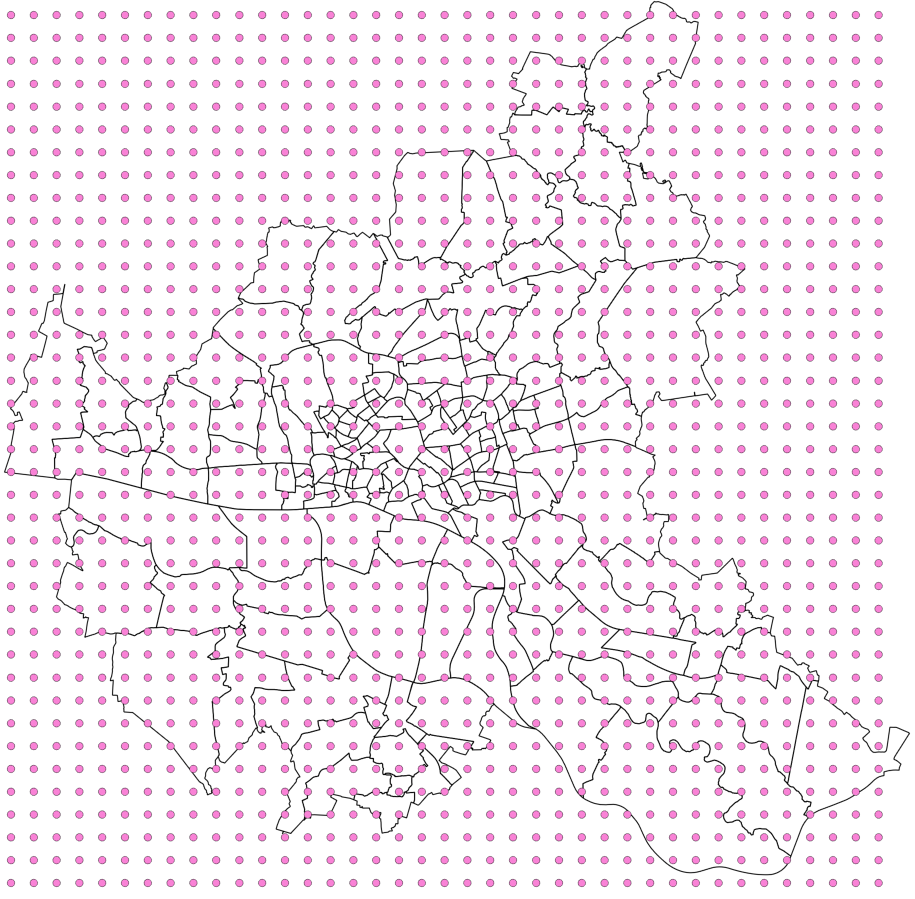
\includegraphics[scale=0.7]{Figures/Recommendation_map/Recommendation_Grid_Centroids.png}
\centering
\caption{Recommendation grid centroids}
\label{fig:Recommendation_Grid_Centroids}
\end{figure}

Since the grid centroids were created to a square map around Hamburg, not all grid centroids were located within the boundaries of Hamburg. Therefore, the centroids were filtered to those on the map of Hamburg in QGIS and joined with the city districts, on which they were located, as displayed in figure \ref{fig:Recommendation_Grid_Centroids_reduced}.

\begin{figure}[h]
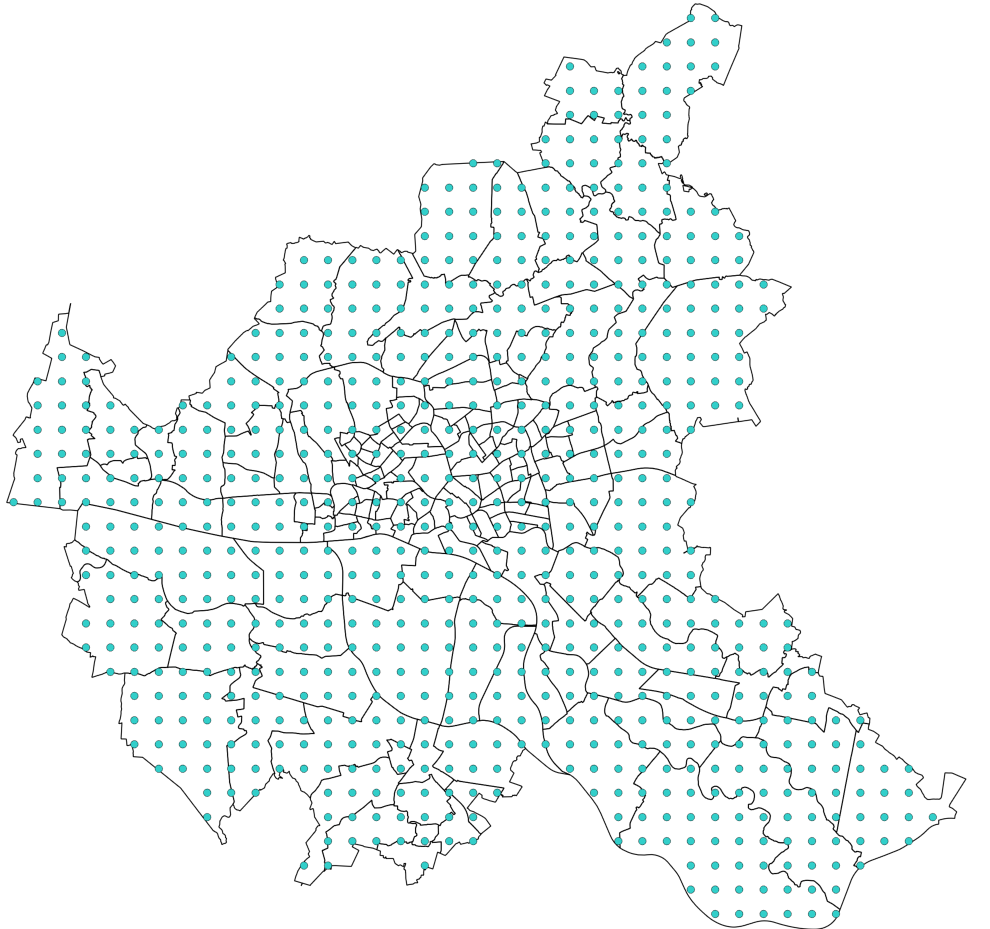
\includegraphics[scale=0.7]{Figures/Recommendation_map/Recommendation_Grid_Centroids_reduced.png}
\centering
\caption{Recommendation grid centroids filtered with the Hamburg districts}
\label{fig:Recommendation_Grid_Centroids_reduced}
\end{figure}

In the next step, all the features for the recommendation centroids were collected together and were used to predict the success contributions of these locations. The location-dependent features, which are described in section \ref{sec:Feature_selection}, were mainly location-dependent and could be either extracted from the city district that a centroid was in or calculated, like the distance to the next water bodies or the restaurant density in these centroids.

Two factors, however, were not location-dependent and multiple values had to be fed into the feature sets to predict the success of each variation. One of these factors was the price level as a category from price level 1 to price level 5. Predictions for all of these price levels were created. However, most frequently price level 2 was selected as the price level with the highest success contribution, independent of the other features. As the price has a relatively high influence on restaurant success, the highest success contributing price was to be predicted for every point. The second factor, which was included and which was not location-dependent, was the category of the restaurant, for which a location should be found. As there were many restaurants with different categories with the same success contributions, the ``best'' restaurant category was not predicted but taken as an input parameter. The business question that the recommendation map therefore answers is if a customer wants to open a restaurant of a specific category, e.g., a Vietnamese restaurant, where the location with the highest success contribution would be. For this, the restaurant types with the seven highest frequencies in Hamburg were taken into account and used for an exemplary analysis. The seven most frequent categories are presented in table \ref{table:category_frequencies}. For each of these most common categories, a recommendation map was created.

\begin{table}[h!]
\begin{center}
\begin{tabular}{| c | c |}
\hline
 restaurant category & number of restaurants \\
 \hline
 cafes & 520 \\ 
 german & 391 \\  
 italian & 387 \\    
 hotdogs & 245 \\
 greek & 223 \\
 pizza & 193 \\
 kebab & 165 \\
 \hline
\end{tabular}
\caption{Restaurant category frequencies in Hamburg}
\label{table:category_frequencies}
\end{center}
\end{table}

In the Python file ``analysis.py'', predictions for all recommendation centroids were created in two for-loops that replicate the projections for all seven top categories and all price levels. Afterward, the prediction values were saved together with their locations and their feature values into \ac{csv} files that could later be loaded into QGIS. Additionally, the top five spots for every category map were extracted and saved into a separate \ac{csv} file to be able to highlight them on the maps.

For the creation of the recommendation maps, for each category, the recommendation centroids were loaded onto the QGIS Hamburg map together with their predicted success contribution and the additional features. These recommendation centroids were then saved in the same color and additionally converted to a raster that would show the success contribution as a color on the map. To save this raster, the attribute field was set to the predicted success, and the raster resolution was set to 1,000 units per pixel. The color of the rasters was set to ``Singleband gray'' with a color gradient from black to white meaning the darker a location is, the less success is expected at this location, and the brighter a location gets, the more success is expected. Furthermore, the transparency of the rasters was set to 40\% to be able to see the Hamburg district map in the background. In addition, the top 5 centroids of each category were imported into QGIS and displayed on the map. In figure \ref{fig:Greek_restaurant_success_contribution_map}, the success prediction map for Greek restaurants is shown as an example. Enabling the ``Identify Features'' option after clicking on the recommendation centroids layer of the respective category showed the features in a given location.

\begin{figure}[h]
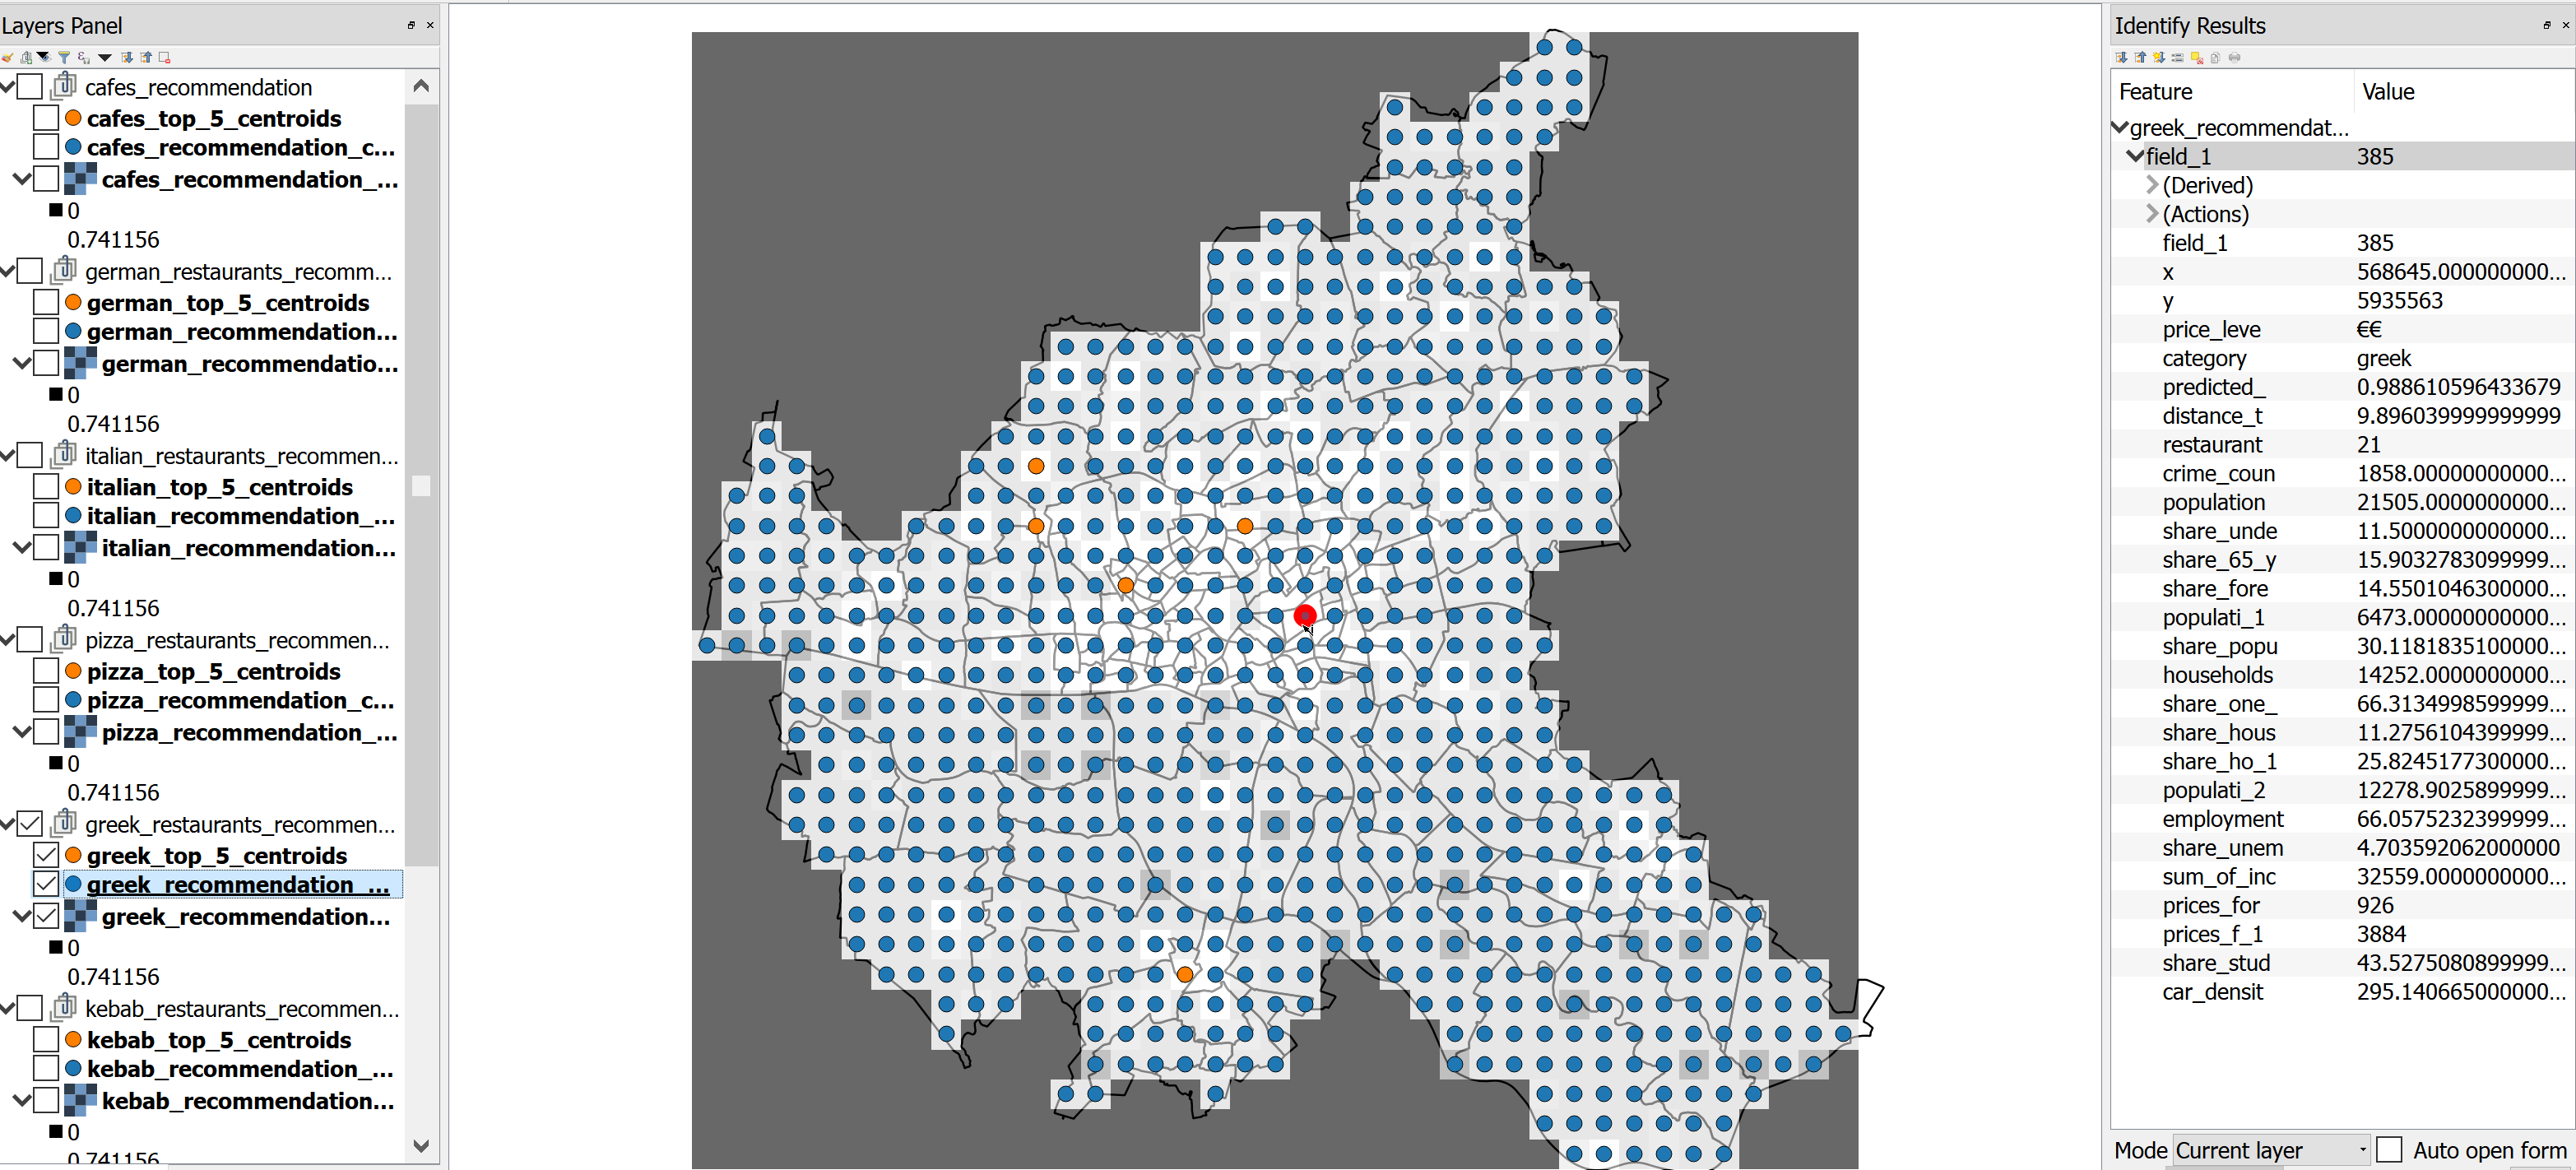
\includegraphics[scale=0.5]{Figures/Recommendation_map/greek_restaurant_recommendation_map.png}
\centering
\caption{Greek restaurant success contribution map}
\label{fig:Greek_restaurant_success_contribution_map}
\end{figure}

\section{Locations for restaurant recommendations for restaurants in Hamburg}

In section \ref{creation_of_recommendation_map}, recommendation maps that indicate the success contribution of all points in Hamburg for a given restaurant category, were created. It was recognized that for the seven most frequent restaurant categories (cafes, German, Italian, hot dogs, Greek, pizza, and kebab), always the same five locations were found to be most success contributing. These five locations are displayed in figure \ref{fig:Top_Five_Locations}. The x and y coordinates on the \ac{etrs89} \ac{crs} are given in table \ref{table:top_five_locations}. The predictions for these five locations are based on all the features, which were used in the \ac{rfr}. Further, most of the times price level 2 was predicted as the price category with the highest success contribution.

\begin{table}[h!]
\begin{center}
\begin{tabular}{| c | c |}
\hline
x & y \\
 \hline
 562645 & 5936563 \\ 
 566645 & 5938563 \\  
 564645 & 5923563 \\    
 559645 & 5938563 \\
 559645 & 5940563 \\
 \hline
\end{tabular}

\caption{Top 5 locations for restaurant success according to random forest predictions (ETRS89)}
\label{table:top_five_locations}
\end{center}
\end{table}

\begin{figure}[h]
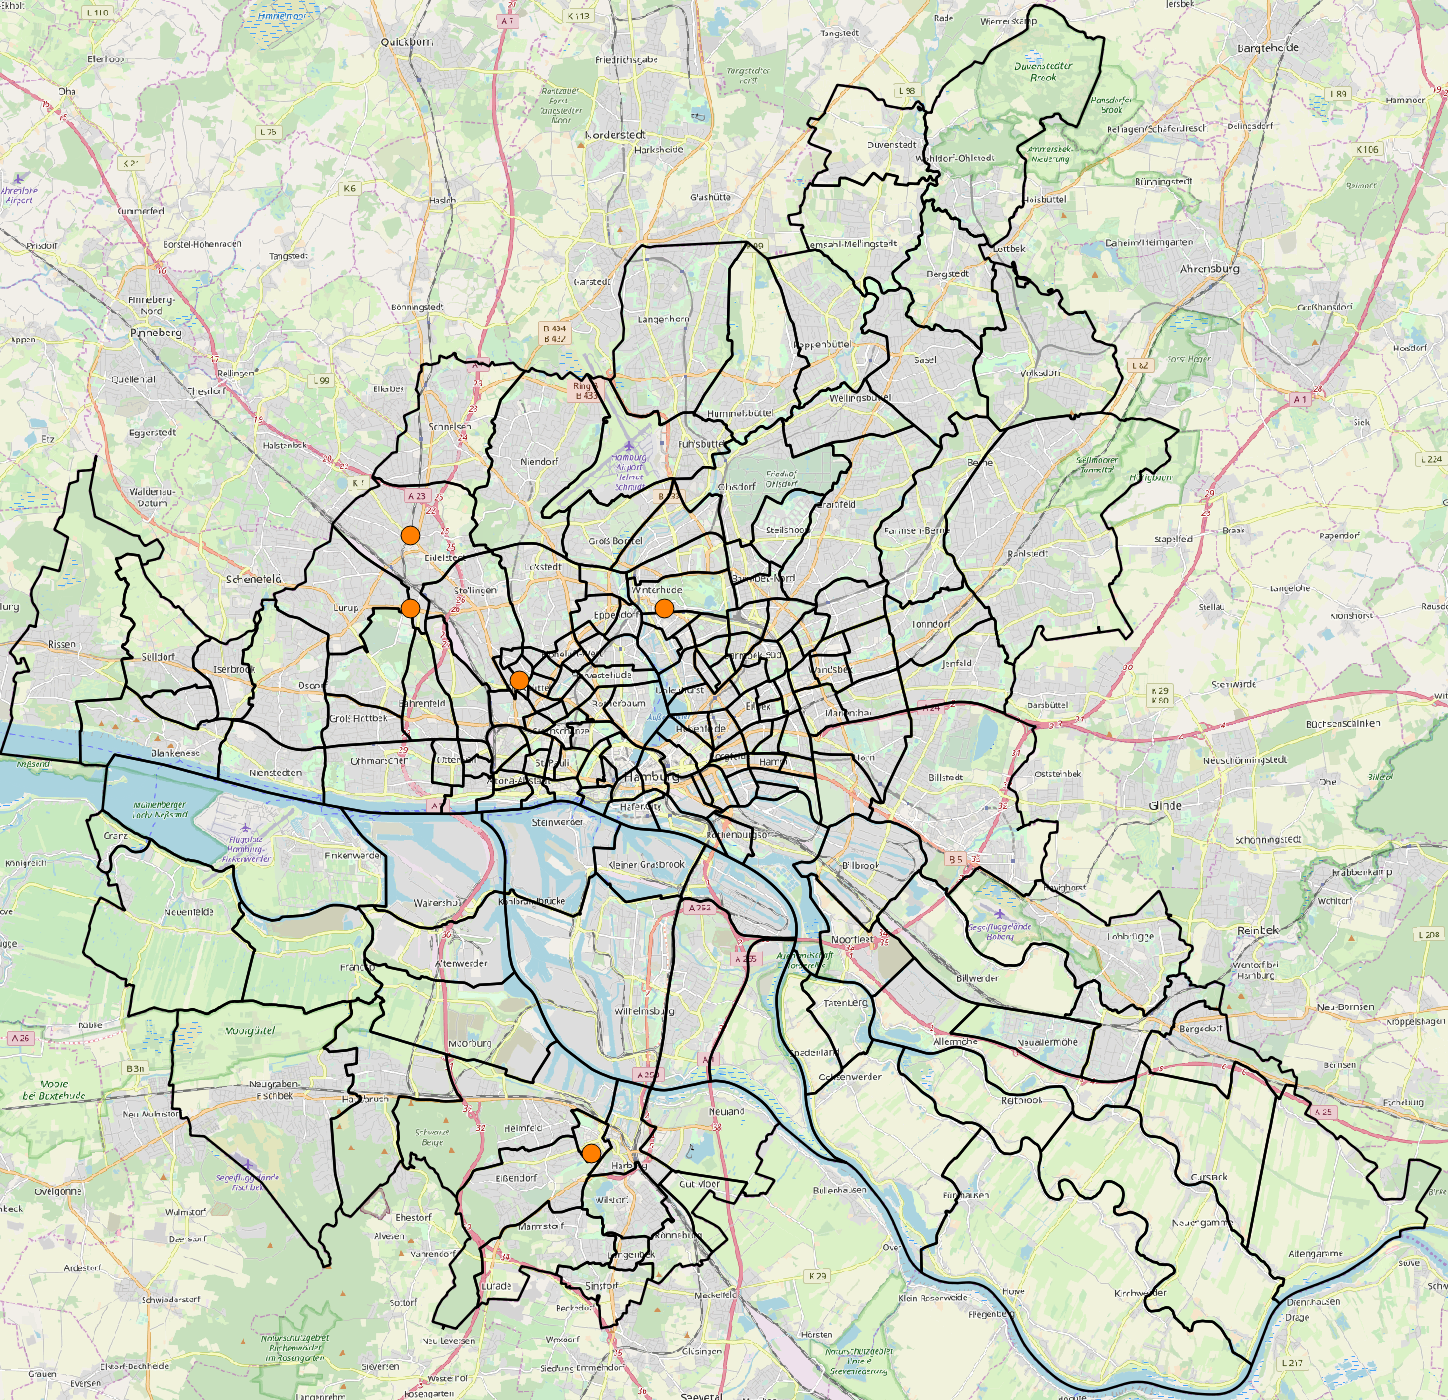
\includegraphics[scale=0.5]{Figures/Recommendation_map/Top_Five_Locations.png}
\centering
\caption{Top 5 locations for restaurant success according to random forest predictions}
\label{fig:Top_Five_Locations}
\end{figure}


\chapter{Discussion}
\lhead{\emph{Discussion}}
\label{Discussion}

This chapter visualizes and discusses the patterns and findings of the data analysis conducted with the machine learning regression model developed in this paper.

\section{Exploratory data analysis}
\label{Exploratory_data_analysis}

\textbf{1.	Variable Importance}

\begin{figure}[h]
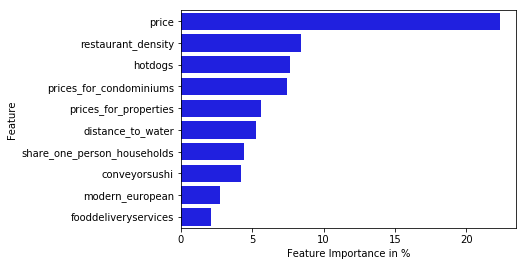
\includegraphics[scale=0.7]{Figures/Exploratory/feature_importance_barplot.png}
\centering
\caption{Feature importance for random forest predictions}
\label{fig:feature_importance_barplot}
\end{figure}

Figure \ref{fig:feature_importance_barplot} shows the features which had high importance in the random forest prediction. The overview indicates that the price is the most important feature for the success and failure of a restaurant. Further, the density of restaurants, type of food like hot dogs, the price of condominiums, the distance from water and the share of households with one person play a significant role in the success of the restaurants.

\textbf{2.	Price level}

\begin{figure}[h]
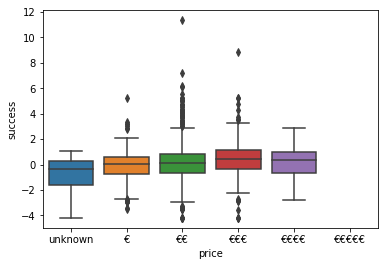
\includegraphics[scale=0.7]{Figures/Exploratory/boxplot_price_levels.png}
\centering
\caption{Boxplot diagram of restaurant price levels with success}
\label{fig:boxplot_price_levels}
\end{figure}

Figure \ref{fig:boxplot_price_levels} shows the relationship between the price level and the success of the restaurants in the dataset. It can be seen that the median of boxplots for different price levels increases together with the price level and it starts decreasing with a higher price level than 3. It indicates that the price level of restaurants in the extracted data correlated with their success. This could mean that there are consumers willing to pay high prices for restaurants and leave a good review if they are satisfied and consider the prices justified. With price level 4, the overall restaurant success decreases, which could indicate either that too few consumers are willing to pay prices in this range or that the consumers were not satisfied with the restaurants’ offerings. Price level 5 showed no records, which may either indicate a lack of demand in this price range or a lack of restaurants able to service a justified offering for price level 5.

\textbf{3.	Distance to Water}
 
\begin{figure}[h]
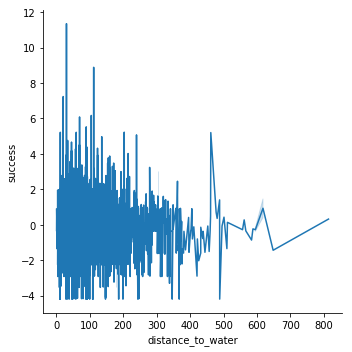
\includegraphics[scale=0.7]{Figures/Exploratory/lineplot_distance_to_water.png}
\centering
\caption{Restaurant distance to water and success}
\label{fig:lineplot_distance_to_water}
\end{figure}
 
From figure \ref{fig:lineplot_distance_to_water}, it can be seen that most of the restaurants are located within a range of 400 meters from water spots and that there is a huge variation in the success rate of these restaurants. However, the number of restaurants with a higher success rate is in the majority present in restaurants within a range of 200 meters near water spots.

\textbf{4.	Condominiums Price}
 
\begin{figure}[h]
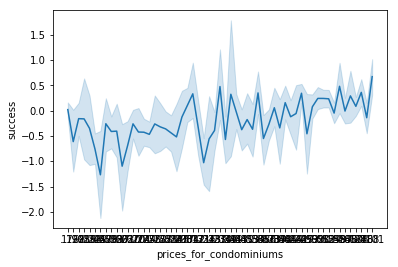
\includegraphics[scale=0.7]{Figures/Exploratory/lineplot_prices_for_condominiums.png}
\centering
\caption{Condominium Price and success}
\label{fig:lineplot_prices_for_condominiums}
\end{figure}
 
Figure \ref{fig:lineplot_prices_for_condominiums} shows that the price of condominiums and success of the restaurants in the dataset are slightly positively correlated, although this correlation varies strongly. This could mean that the prices of condominiums are high in the area of high restaurant demand and supportive markets, such as downtown areas, which may lead to high restaurant success rates.

\textbf{5.	Income}
 
\begin{figure}[h]
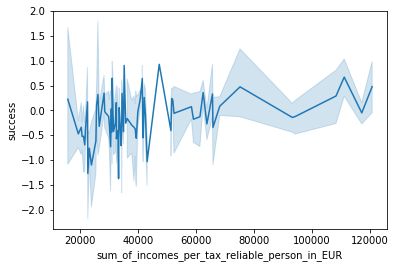
\includegraphics[scale=0.7]{Figures/Exploratory/lineplot_income.png}
\centering
\caption{Income and success}
\label{fig:lineplot_income}
\end{figure}

From figure \ref{fig:lineplot_income}, it can be seen that the success of restaurants in the extracted data is proportional to the income of the inhabitants in the vicinity of a restaurant. Also, it could indicate that the number of restaurants is significantly less in extremely high-income areas of more than 70,000 euros per inhabitant and year, but still these restaurants have a high success rate.

\textbf{6.	Restaurant density}
 
\begin{figure}[h]
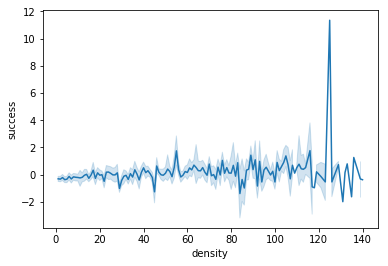
\includegraphics[scale=0.7]{Figures/Exploratory/lineplot_restaurant_densities.png}
\centering
\caption{Restaurant density and success}
\label{fig:lineplot_restaurant_densities}
\end{figure}

Figure \ref{fig:lineplot_restaurant_densities} shows that the overall success rate does not vary much with the increase in restaurant density. This could be due to the positive effect of restaurant density through a high demand of the market providing enough customers to all restaurants and the negative effect of competition through other restaurants.

\textbf{7.	Population Density}
 
\begin{figure}[h]
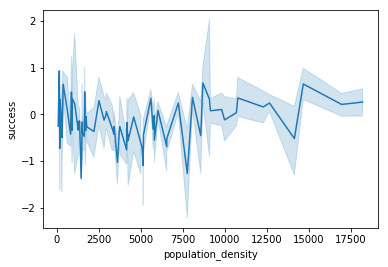
\includegraphics[scale=0.7]{Figures/Exploratory/lineplot_population_density.png}
\centering
\caption{Population density and success}
\label{fig:lineplot_population_density}
\end{figure}

Figure \ref{fig:lineplot_population_density} shows that the frequency and success rate of restaurants are higher in the low population density area with less than 2,500 inhabitants. This could be due to the reason that areas in the vicinity of city centers with more commercial activity are usually less residential areas. Additionally, it can be seen that the frequency of restaurants in high population density areas with more than 9,000 inhabitants is lower, but the success rate tends to be higher which could be due to the residential area.

\textbf{8.	One-Person Households}
 
\begin{figure}[h]
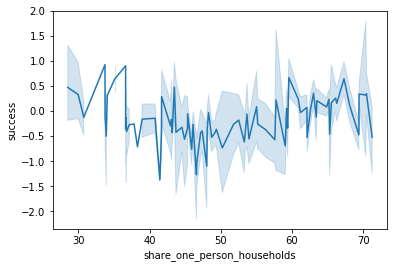
\includegraphics[scale=0.7]{Figures/Exploratory/lineplot_one_person_households.png}
\centering
\caption{One-person households and success}
\label{fig:lineplot_one_person_households}
\end{figure}

It can be seen from the value frequency in figure \ref{fig:lineplot_one_person_households} that the number of restaurants is higher in areas with a high share of one-person households of more than 45\%. Additionally, the success rate tends to be higher in the areas with high shares of one-person households. This could be due to people in one-person households having their meal more frequently outside with others in company.

\section{Discussion of results}
\label{discussion_of_results}

In this paper, a recommendation map for restaurants together with beneficial locations for new restaurants could be created. This recommendation map answers to any potential restaurant owner the question of where to place a restaurant. Since the $R^2$ and Adjusted $R^2$ values of the \ac{rfr} were positive, the predictions can bring value to the decision of a restaurant placement. Furthermore, the features that were used for the prediction of the success, can be explained to potential restaurant owners, which enables them to evaluate these values for their location decision themselves.

However, the interrelation of 21 features and the restaurant category as input values for a location decision may be too complex for a human being to undertand. Since the final model of 1,0000 weighted decision trees within the random forest regressor is also too complex to understand for human beings, the grounds for the prediction of restaurant success are difficult to understand. This may leave a potential restaurant owner with a decision on a location for a new restaurant without the understanding of why this location was chosen. The feature importance and exploratory data analysis presented in section \ref{Exploratory_data_analysis} present the relationships between important features of the random forest regressor, but a decision model with more than 22 features is challenging to understand with two- or three-dimensional models than can be visually understood by human beings.

Additional to the problem of model simplicity, the success of a restaurant is not only explainable by its location. As described in section \ref{viability_factors}, there are more factors to the viability of a restaurant than its location. This is recognizable in the $R^2$ and Adjusted $R^2$ values for the test sets of ca. 0.1. These values are high enough to add value to a placement decision, but are not high enough to rely the restaurant success solely on these predictions.

A challenge to the prediction of restaurant success, furthermore, was the success metric itself. Restaurant success would usually be measured by financial figures like the profit, revenue or customer count of restaurants. In lack of this data, a success metric was created based on the Yelp reviews count and rating, which itself would be a valuable feature to predicting a restaurant's success. As the reviews of a restaurant both are a mirror of the restaurant success, but itself are a feature that can influence the restaurant's success, this metric is applicable for this paper, but has limitations. These limitations may also stem from the fact that a restaurant, which has highly rated and many reviews, but which does not work profitably, would be seen as a successful restaurant.

Another limitation resulting from the given data is the restriction of the restaurant location analysis to one city. As one city's feature values may be closer to each other than in the comparison to other cities or villages in the same or other countries, data from more cities would be beneficial to the prediction of success. However, as the provision and measurement of data is not performed equally in different countries and not even within Germany, such an analysis would suffer from a questionable comparability and availability of data. Nevertheless, the regression model found in this paper would benefit from future research into the verification of the model and review of the comparability of available data sources of other areas for features used in this paper.

Despite all these challenges, the predictions of restaurant success and creation of a recommendation may be a beneficial technique for restaurant owners, e.g., to start or to verify their own location analysis.

\chapter{Conclusion}
\lhead{\emph{Conclusion}}
\label{Conclusion}

This paper aims at a restaurant location analysis in Hamburg and strives to find a method of selecting a beneficial location for the success of restaurants. For this, the correlation of location-dependent features to restaurant success has been analyzed and applied to a random forest regressor, which can predict the contribution to a restaurant success from the features given by a location. With this, a map of Hamburg could be created that presents recommended locations for the placement of a restaurant given a restaurant category. Five locations were named, which are predicted as beneficial to restaurant success on any of the seven most frequent restaurant categories in Hamburg.

Multiple challenges were found with the used method of analyzing data from a review portal and from city-related sources to predict success for specific locations. Among these challenges was the complexity of \ac{rfr} that impedes a clear understanding of the decision basis for choosing a location as beneficial for opening a restaurant. An exploratory data analysis in the review of two-dimensional graphs of features against each other supported the understanding but suffered high variance and the little contribution that each of the attributes presents in the overall complex prediction model. Moreover, as location-dependent features are only one part of the factors for restaurant success, just a contribution to restaurant success by locations could be recognized. Further, the restaurant success metric was a deducted metric from review portal reviews and, while presenting a perspective on a restaurant's success, review portal reviews are not regularly employed as the leading indicator for restaurant success.

The regression model for location contribution to restaurant success was applied to the metropolis of Hamburg. As differences of environmental factors may be lower within a city than to locations outside, future research could be conducted to cross-verify the model found for Hamburg in other areas. Another benefit from such an analysis would be the verification of the availability of data sources that could be found in Hamburg.

Notwithstanding the challenges of this research and the merger of multiple non-related data sources, a contribution of the location to the success of restaurants could be found and a success contribution prediction could be applied to new positions within Hamburg. These findings may aid restaurant owners in their choice of a location, e.g., at the start of their location search analysis. Additionally, it may support future research in the exploration of location factors influences to restaurant success comprising which features can be used and how the data for these can be retrieved. In this manner, this paper adds knowledge about the composition of success factors to restaurant location analyses and may represent one part of the way to greater clarity in this area.

%% ----------------------------------------------------------------
% Now begin the Appendices, including them as separate files

%\addtocontents{toc}{\vspace{2em}} % Add a gap in the Contents, for aesthetics

%\appendix % Cue to tell LaTeX that the following 'chapters' are Appendices

%\input{Appendices/AppendixA}	% Appendix Title

%\input{Appendices/AppendixB} % Appendix Title

%\input{Appendices/AppendixC} % Appendix Title

\addtocontents{toc}{\vspace{2em}}  % Add a gap in the Contents, for aesthetics
\backmatter

%% ----------------------------------------------------------------
\label{Bibliography}
\lhead{\emph{Bibliography}}  % Change the left side page header to "Bibliography"
\bibliographystyle{unsrtnat}  % Use the "unsrtnat" BibTeX style for formatting the Bibliography
\bibliography{Bibliography}  % The references (bibliography) information are stored in the file named "Bibliography.bib"

\end{document}  % The End
%% ----------------------------------------------------------------